\chapter{Bifurcation theory}
\section{Versality}

According to Theorem \ref{theo:2.43}, typical vector fields on a compact 2-dimensional manifold $M$ are orbitally structurally stable. If we denote by $\mathcal{X}$ the infinitely dimensional space of all vector fields on $M$ (given a class and with a suitable topology that we will not talk about), then the subset $\Sigma$, called the \textit{bifurcation set}, of the space $\mathcal{X}$  consisting of fields that are not orbitally structurally stable, should have codimension $\geq 1$. It should be expected that this subset $\Sigma$ is generally smooth, but may have irregular points (as in Figure \ref{fig:3.1}). The last points should correspond to vector fields which have more complex singularities than those corresponding to typical points from $\Sigma$.

\begin{figure}[!ht]
	\centering
	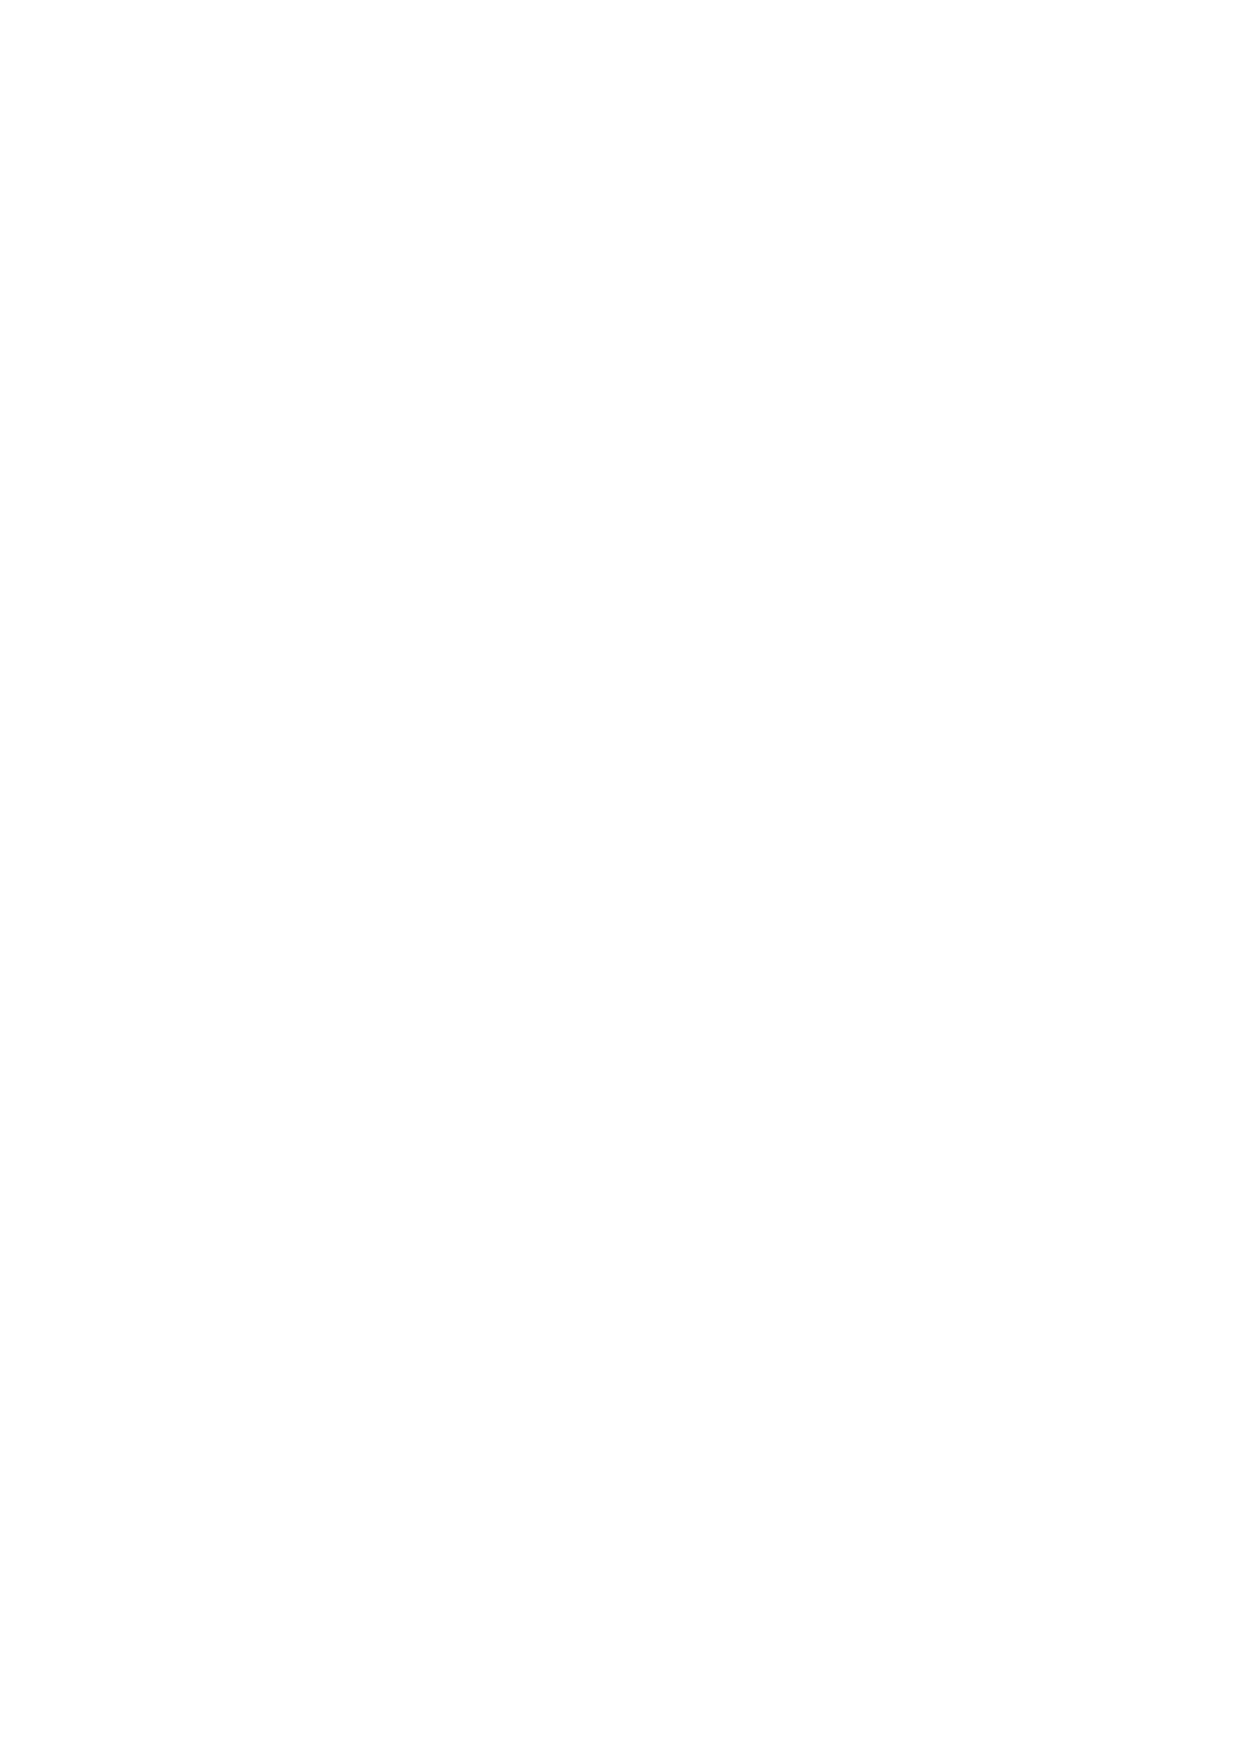
\includegraphics [scale=1]{jtr31}
	\caption{Bifurcation set.}
	\label{fig:3.1}
\end{figure}

If we randomly select a field from $\mathcal{X}$, then with probability 1 it will be outside of the set $\Sigma$. But the whole family $\left\{ v_{\lambda }\right\} _{\lambda \in \mathbb{R}}$ of vector fields is a curve in $\mathcal{X}$ and can already cross the hypersurface $\Sigma$. We also expect that, for a typical family, the corresponding curve will cross the $\Sigma$ hypersurface at the angle and at typical points of this hyperplane (see Figure \ref{fig:3.1}).

The bifurcation theory is concerned with the study of both the geometry of the bifurcation set $\Sigma$ and the behavior of the multi-parameter families of the vector fields. We will limit ourselves to 1-parameter families.

Pay attention to one more aspect of this situation. In space $\mathcal{X}$ there exists a group $\mathcal{G}$ of orbital equivalence and the subdivision $\Sigma$ is invariant in relation to that action. It is therefore necessary to link the analysis of 1-parameter families $\left\{ v_{\lambda }\right\} $ to the action of group $\mathcal{G}$. V. Arnold in \cite{Ar2} introduced once and for all the definitions in this field and the following definitions come from him.\footnote{This philosophy also works in other general situations. For example, where $\mathcal{X}$ is a space of functions $f$ on manifolds, and $\mathcal{G}$ is the group of diffeomorphisms $h$ of manifold with the function $f\longmapsto f\circ h.$ Likewise, $\mathcal{X}$ can be a space of the diffeomorphisms $f$ of the manifold $M$ and the group $\mathcal{G}$ of the diffeomorphisms on $M$ can be obtained by composition: $f\longmapsto h\circ f\circ h^{-1}$.}

\begin{definition}
	The two families $\left\{ v_{\lambda }\right\} _{\lambda
	\in J}$ and $\left\{ w_{\lambda }\right\} _{\lambda \in J}$, $J\subset \mathbb{R}$, of the vector fields on $M$ are \textbf{orbitally equivalent} if for every $\lambda \in J$, the fields $v_{\lambda }(x)$\ and $w_{\lambda }(x)$ are orbitally equivalent by the homeomorphism $h (x)$, which depends in a continuous manner on the parameter $\lambda$.
	
	We say that the family $\left\{ w_{\nu }\right\} _{\nu \in K}$ is \textbf{induced} from $\left\{ v_{\lambda }\right\} _{\lambda \in J}$ if there exists a continuous mapping $\varphi :K\longmapsto J$ such that
	$$
	w_{\nu }=v_{\varphi (\nu )}.
	$$
	
	The family $\left\{ v_{\lambda }\right\} _{\lambda \in \left( \mathbb{R}%
	,0\right) },$ with the given $v_{0}$, is \textbf{versal} if any other family $\left\{ w_{\nu }\right\} _{\nu \in \left( \mathbb{R}%
	,0\right) }$ with $w_{0}=v_{0}$ is orbitally equivalent to a family induced from the family $\left\{ v_{\lambda }\right\} .$
\end{definition}

\begin{example}
	Family $\dot{x}=\nu ^{2}+x^{3}$ is induced from family $\dot{x}=\lambda +x^{3}$ with the help of the change of variables $\lambda
	=\varphi (\nu )=\nu ^{2}.$
\end{example}

\begin{example}\label{example:3.3}
	Let's model the vector field family
	\begin{equation}
	\label{3.1}
	\dot{x}=v_{\lambda }(x)=\lambda +x^{2}.
	\end{equation}
	The corresponding phase portraits are shown in Figure \ref{fig:3.2}.
	
	Let us now take any family of form
	\begin{equation}
	\label{3.2}
	\dot{x}=w_{\mu }(x)=x^{2}+\mu \tilde{w}(x,\mu )=:f(x,\mu ),
	\end{equation}
	where $\tilde{w}(x,\mu )$  is a smooth function in a neighborhood of $x=\mu
	=0 $. We claim that 
	\begin{figure}[!ht]
		\centering
		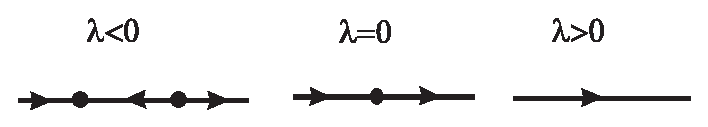
\includegraphics [scale=1]{jtr32}
		\caption{Phase portraits.}
		\label{fig:3.2}
	\end{figure}

	\emph{for every $\mu$ the vector field $w_{\mu }$ has either 1 or 2 or 0 singular points in a neighborhood of $x = 0$.}\\
	To see this, consider the equation
	$$
	g(x,\mu )=0,
	$$
	where $g(x,\mu )=f_{x}^{\prime }(x,\mu ).$ Since $f_{xx}^{\prime
	\prime }(0,0)\not=0,$ then $g_{x}^{\prime }(0,0)\not=0,$ and from the Implicit Function Theorem there exists a smooth function $\psi (\mu )$ such that the equation $g(\psi (\mu ),\mu )\equiv 0$ is satisfied. This means that point
	$$
	x_{\mu }=\psi (\mu )
	$$
	\begin{figure}[!ht]
		\centering
		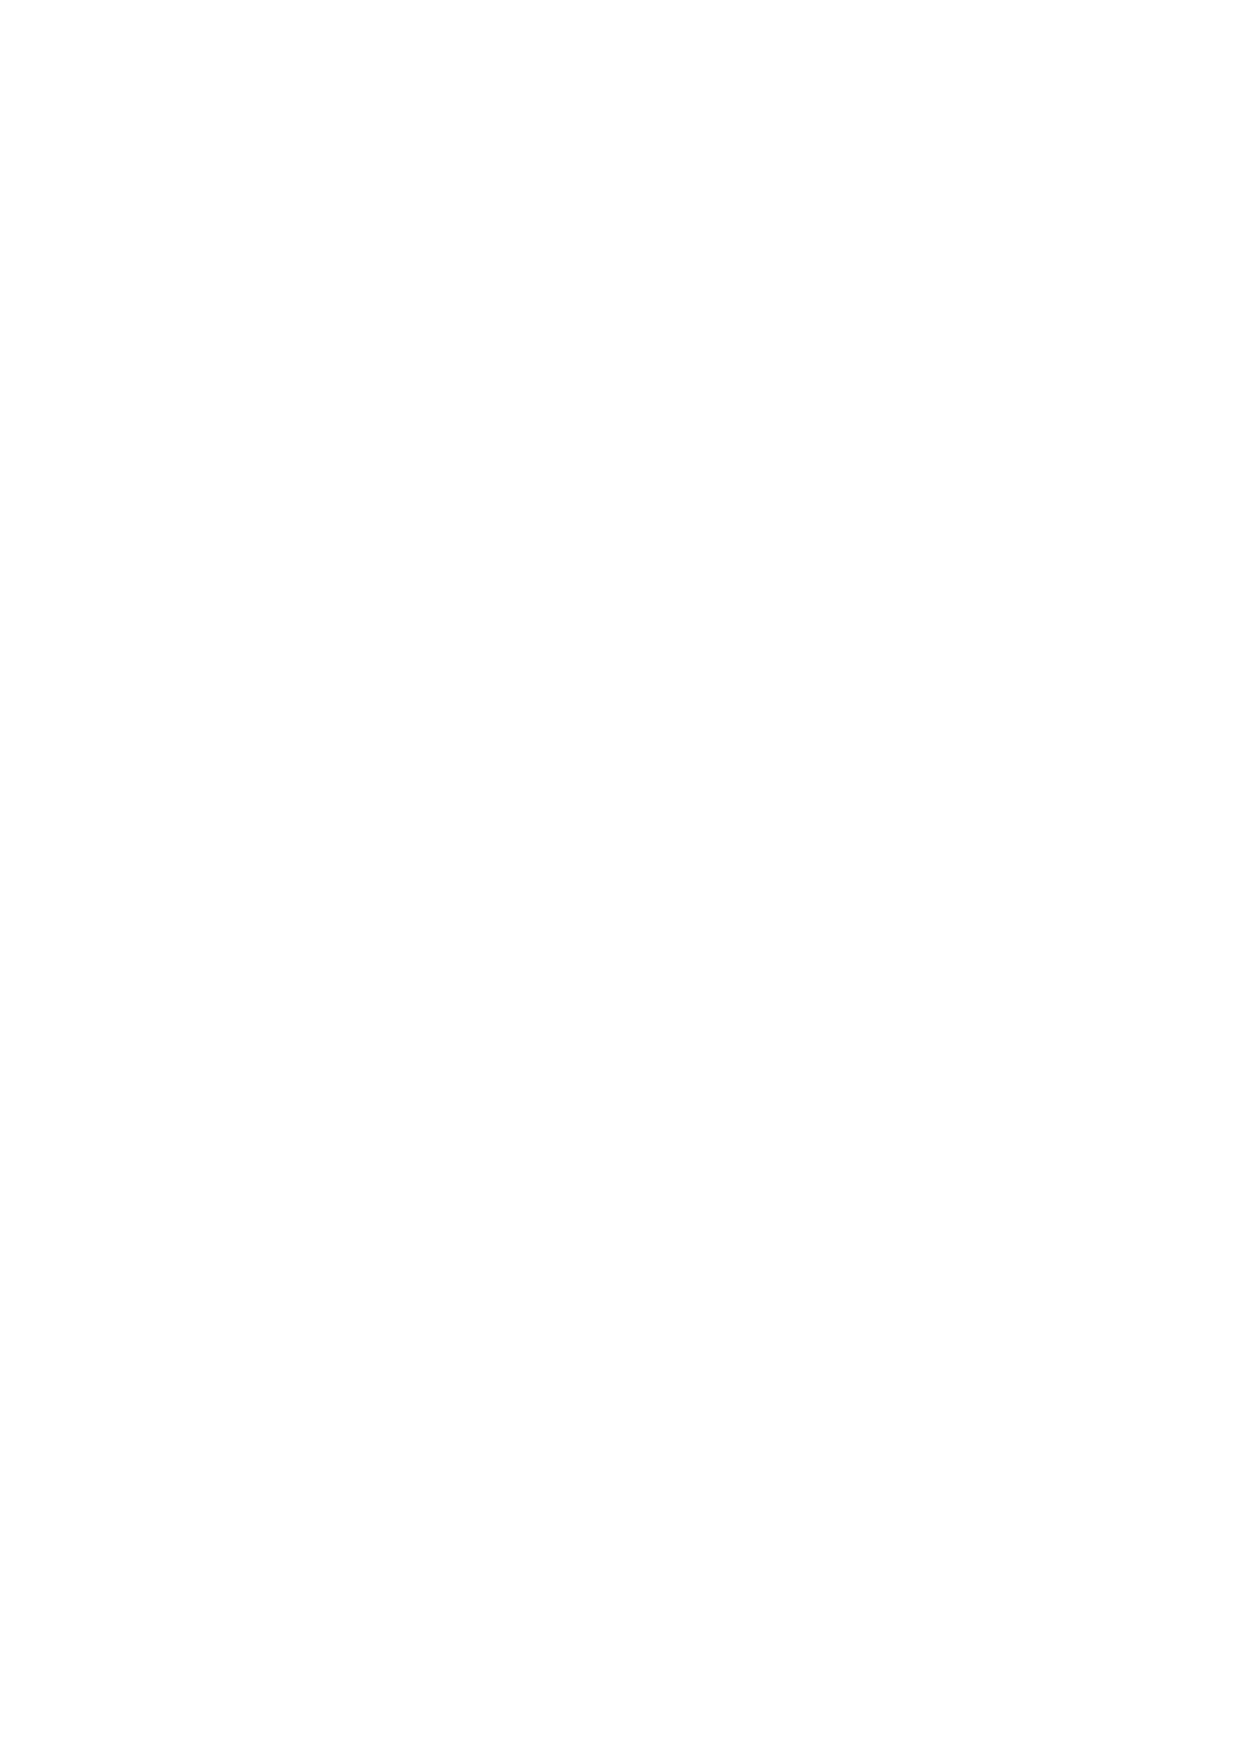
\includegraphics [scale=1]{jtr33}
		\caption{Right-side graphs.}
		\label{fig:3.3}
	\end{figure}
	is the point of the local minimum of the function $w_{\mu }=f(\cdot ,\mu ):\ \frac{dw_{\mu }}{dx}(x_{\mu })=0.$ We have three possibilities for the value of the field $w_{\mu }$ at point $x_{\mu }$: (i) $w_{\mu }(x_{\mu })=0$, (ii) $w_{\mu }(x_{\mu })<0$, (iii) $w_{\mu
	}(x_{\mu })>0$. In case (i) the field $w_{\mu }$ has no equilibrium points (saddle-node type), in case (ii) the field $w_{\mu }$ has two hyperbolic equilibrium points and in case (iii) there is one equilibrium point (see Figure \ref{fig:3.3}).

	So for every $\mu $, the phase portrait of the field $w_{\mu }$ is topologically equivalent to the phase portrait of the field $v_{\lambda }$ for the corresponding $\lambda$. There is a natural question of whether we can obtain $\lambda =\varphi (\mu )$ and homeomorphisms $h_{\mu }$ that realize an orbital equivalence of $w_{\mu }$ with $v_{\varphi (\mu)}$ so that the dependence on $\mu $ is continuous. It turns out that yes; it means that the family \eqref{3.1} is versal.

	\begin{figure}[!ht]
		\centering
		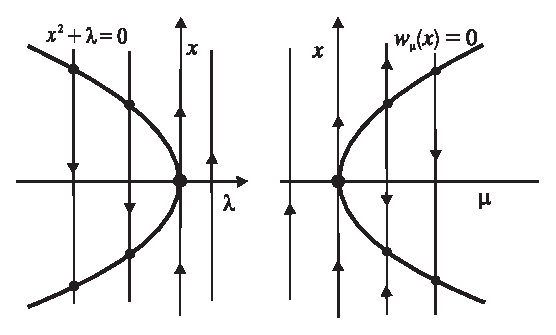
\includegraphics [scale=1.2]{jtr34}
		\caption{Model of family bifurcation and typical family bifurcation.}
		\label{fig:3.4}
	\end{figure}

	In order to convince ourselves, let us first consider the case where
	\begin{enumerate}[(a)]
		\item $\frac{\partial f}{\partial \mu }(0,0)\not=0$ in \eqref{3.2}. Then the curve of the equilibrium point
		$$
		\Gamma :w_{\mu }(x)=f(x,\mu )=0
		$$
		of the field $w_{\mu }$ on the plane of the variables $x,\mu $ is `vertical' and the homeomorphic with a parabola (see Figure \ref{fig:3.4}). Also the parabola is the curve of the equilibrium points $\Delta =\{\lambda =-x^{2}\}$ for the field $v_{\lambda }$.
		
		Depending on the sign of $f_{\mu }^{\prime }(0,0)$ we put $\varphi
		\left( \mu \right) =\mu $ or $\varphi
		\left( \mu \right) =-\mu $; so we can assume that both `parabolas' are oriented the same way. In this case, the homeomorphic constructions $h_{\mu }$, i.e., the homeomorphism of the plane $$
		\left( \mu ,x\right) \longmapsto \left( \mu ,h_{\mu }(x)\right) ,
		$$
		start with the construction of the homeomorphism between the curves of the equilibrium points: $\Gamma \longmapsto \Delta $. Then we extend this homeomorphism continuously to the plane, so that the vertical sections (at $\mu =\textrm{const}$) outside the equilibrium points go to the corresponding vertical sections. It is clear that it is possible to do so.
		\item In the degenerate case, when $f_{\mu }^{\prime }(0,0)=0,$ the curve of the equilibrium points $\Gamma =\{f=0\}$ can be very complex (see Figure \ref{fig:3.5}). But we know that from every straight vertical $\mu =\textrm{const}$ the curve has at most two points of the shear. Let us denote the intersection of $\Gamma _{\mu }$ and $\Gamma$ with such a straight line. Thus the parabolic construction $\mu \longmapsto	\varphi (\mu )$ lies in the parameters $\mu$, for which $\#\Gamma _{\mu }=2$ have gone to the left of $\lambda =0$ and the parameters $\mu$, for which $\#\Gamma _{\mu }=0$ have gone to the right of $\lambda =0$ (with continuity). Then, repeating arguments from case (a), we construct a first the continuous transformation $\left( \mu ,x\right) \longmapsto (\varphi (\mu ),h_{\mu }(x))$ between the $\Gamma $ and $\Delta $ curves and then extend them in a continuous manner with the preservation of the vertical.
	\end{enumerate}
	This also proves that the family $v_{\lambda }(x)=\lambda +x^{2}$ is versal.
	\begin{figure}[!ht]
		\centering
		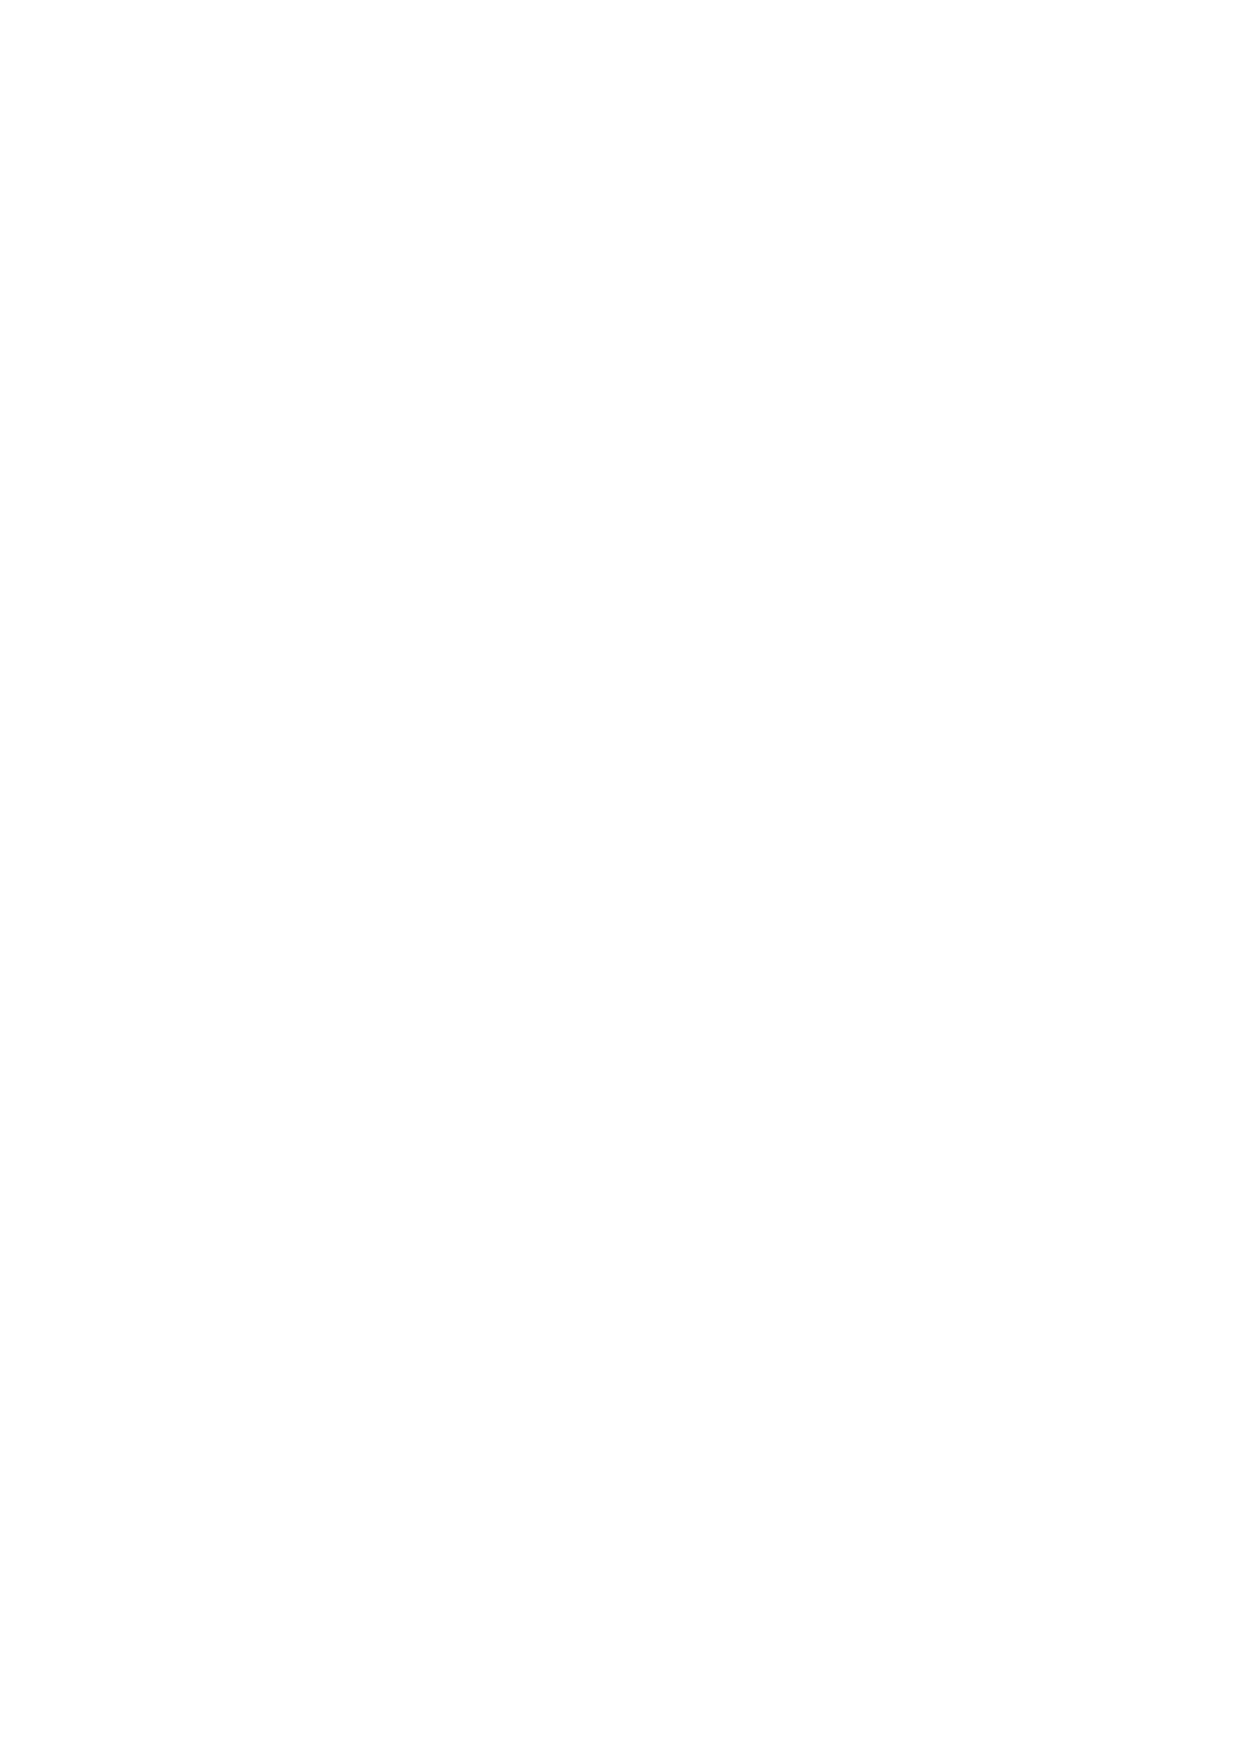
\includegraphics [scale=1]{jtr35}
		\caption{Bifurcation of an atypical family.}
		\label{fig:3.5}
	\end{figure}
\end{example}

\section{Transversality}

A mathematical tool for the exact formulation of bifurcation theory and corresponding theorems is the theory of transversality formulated by the French mathematician R. Thom.

Let $M$ be a $n$-dimensional manifold and let $B\subset M$ be its $k$-dimensional submanifold. In addition, let $A$ be a $m$-dimensional manifold and 
$$
f:A\longmapsto M
$$
will be a differential mapping (with sufficient class of differentiability). In the case of compact manifolds $A$ and $M$ in the space $C^{k}(A,M)$ the natural topology is introduced (which will not be squeezed).
 
 \begin{definition}
 	We say that \textbf{the mapping $f$ is transversal to the submanifold $B$}, if for every point $x\in A$ such that $y = f (x) \in B$, the following property is hold
 	$$
 	f_{\ast }T_{x}A+T_{y}B=T_{y}M.
 	$$
 	When $A\subset M$ is a submanifold and $f=id|_{A}$ is an embedding, then we say that \textbf{$A$ is transversal to $B$} if the property
 	$$
 	T_{y}A+T_{y}B=T_{y}M
 	$$
 	is hold for every point $y\in A\cap B$. We have the standard symbols
 	$$
 	f\pitchfork B\text{ \ \ and \ \ }A\pitchfork B
 	$$
 	for transversal properties.
 \end{definition}

\begin{figure}[!ht]
	\centering
	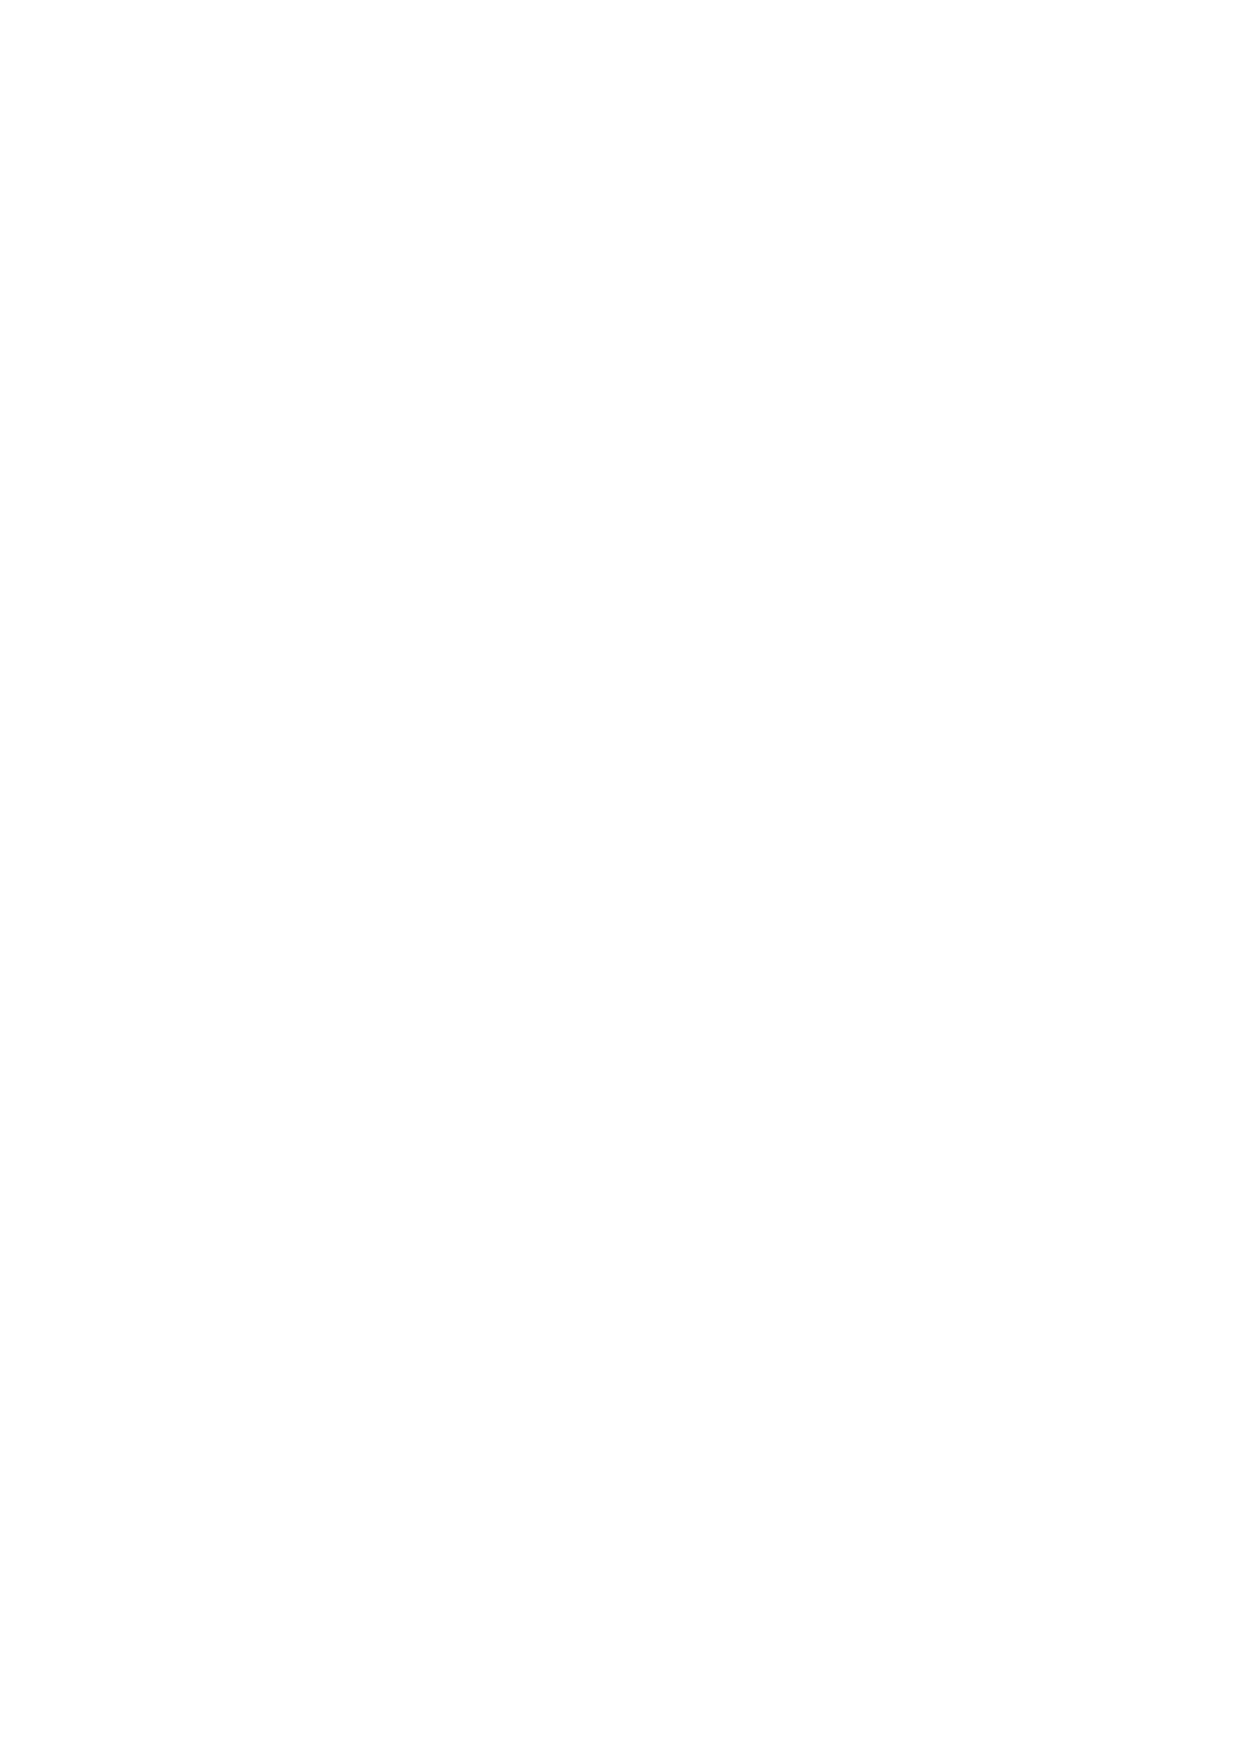
\includegraphics [scale=1]{jtr36}
	\caption{Transversal and non-transversal curves in the plane.}
	\label{fig:3.6}
\end{figure}

\begin{example}
	\begin{enumerate}[(a)]
		\item Let $M=\mathbb{R}^{2}$ and $A\subset M$ and $B\subset M$ be smooth curves. Then  $A\pitchfork B$ when curve $A$ crosses curve $B$ under a non-zero angle (see Figure \ref{fig:3.6}).
		\item Let $M=\mathbb{R}^{3}$, $A\subset M$ be a curve and $B\subset M$ be a submanifold. Figure \ref{fig:3.7} shows cases of transversality and non-transversality.
		\item The case $M=\mathbb{R}^{3}$ and two surfaces $A\subset M$, $B\subset M$ is shown in Figure \ref{fig:3.8}.
		\item When $M=\mathbb{R}^{3}$ and $A\subset M$, $B\subset M$ are curves, then $A\pitchfork B$ if and only if the curves are disjoint.
		\item Let $M=\mathbb{R}^{2}=\left\{ \left( x,y\right) \right\}$, $A = \mathbb{R}^{1}$ and $B=\left\{ x=0\right\} $ and let $f:A\longmapsto M$  be given by the formula $f(t)=(t^{3},0)$. Of course $f(t)\in B$ is only for $t = 0$. But then $f_{\ast }(0)=f^{\prime }(0)=0$. So $f_{\ast		}T_{0}A+T_{(0,0)}B=T_{(0,0)}B\simeq B\not=T_{(0,0)}M$. This example shows the importance of the transversality properties of the mapping to a submanifold.
	\end{enumerate}
\end{example}

\begin{figure}[!ht]
	\centering
	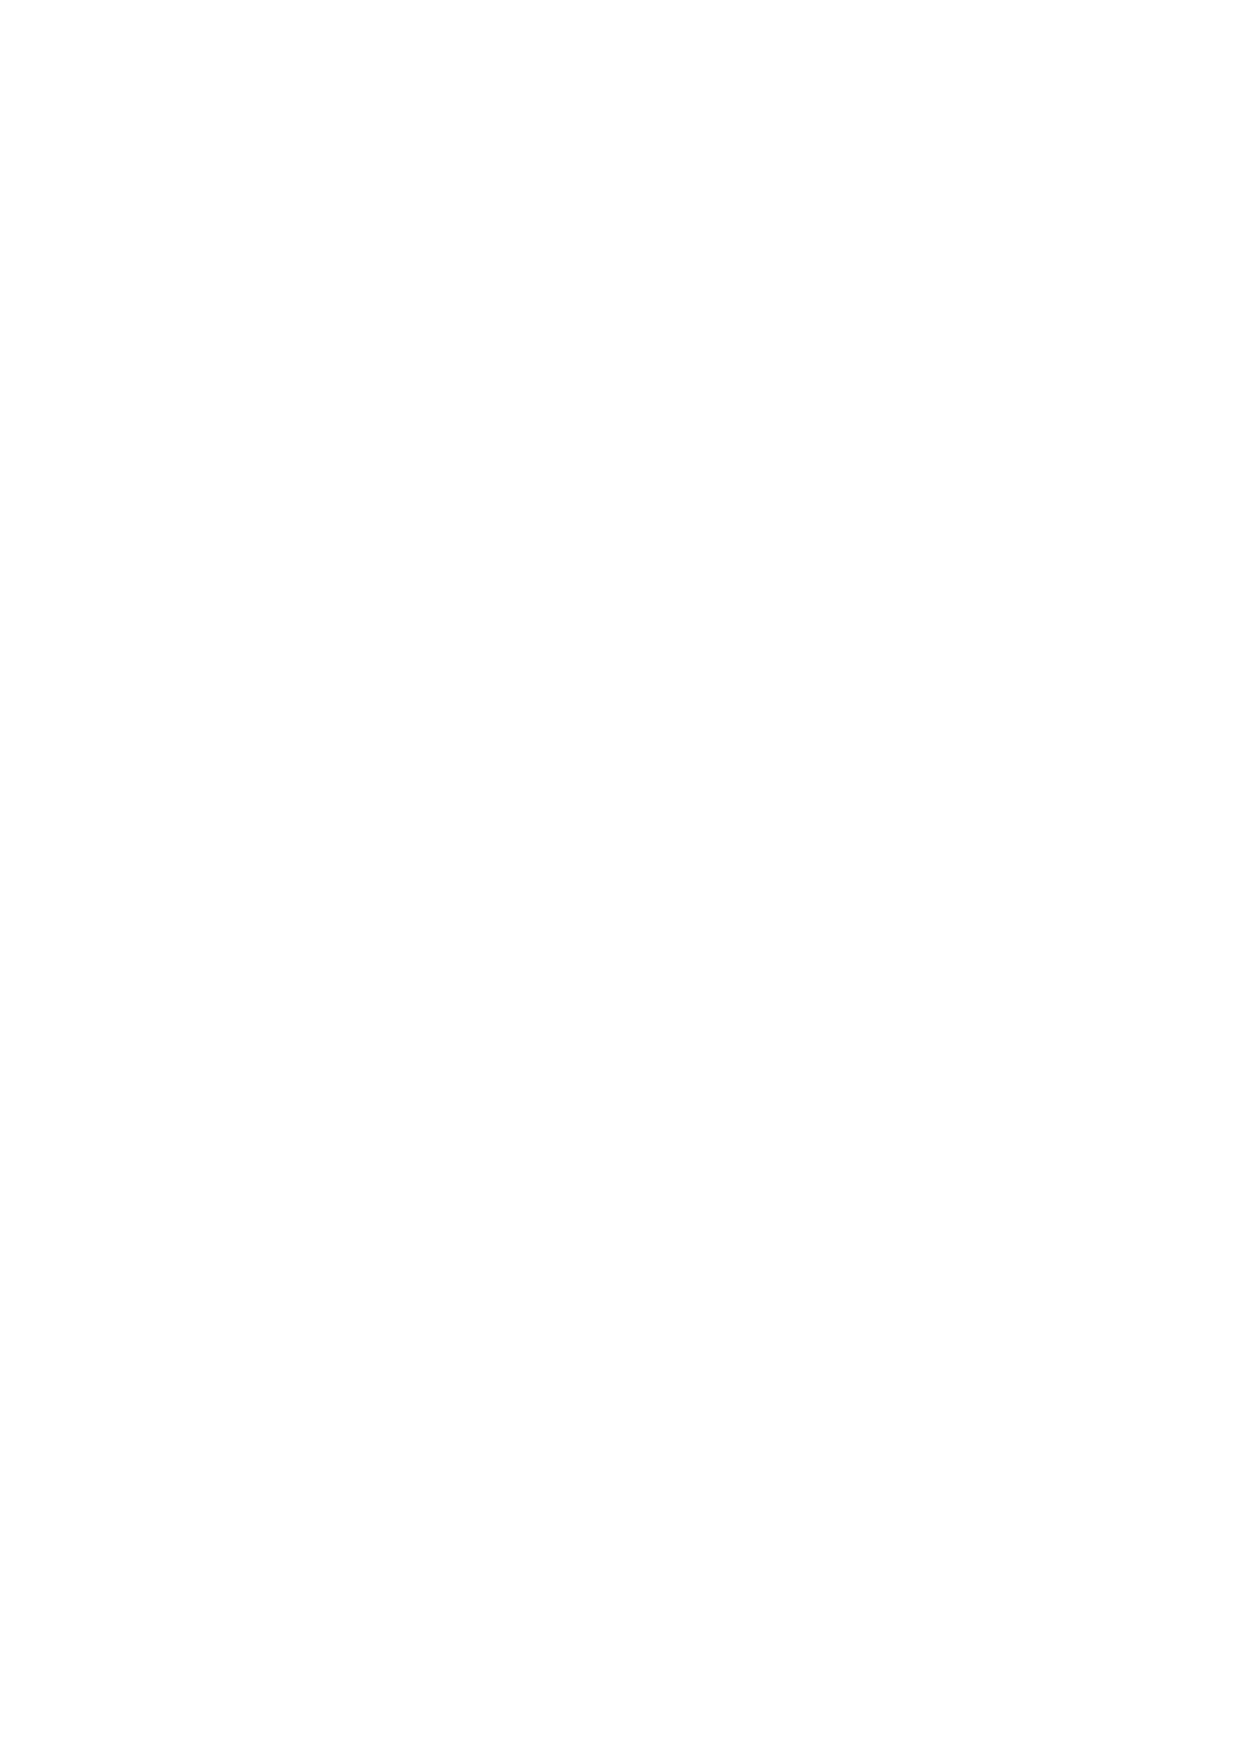
\includegraphics [scale=1]{jtr37}
	\caption{Transversal and non-transversal curve and surface in the space.}
	\label{fig:3.7}
\end{figure}

\begin{figure}[!ht]
	\centering
	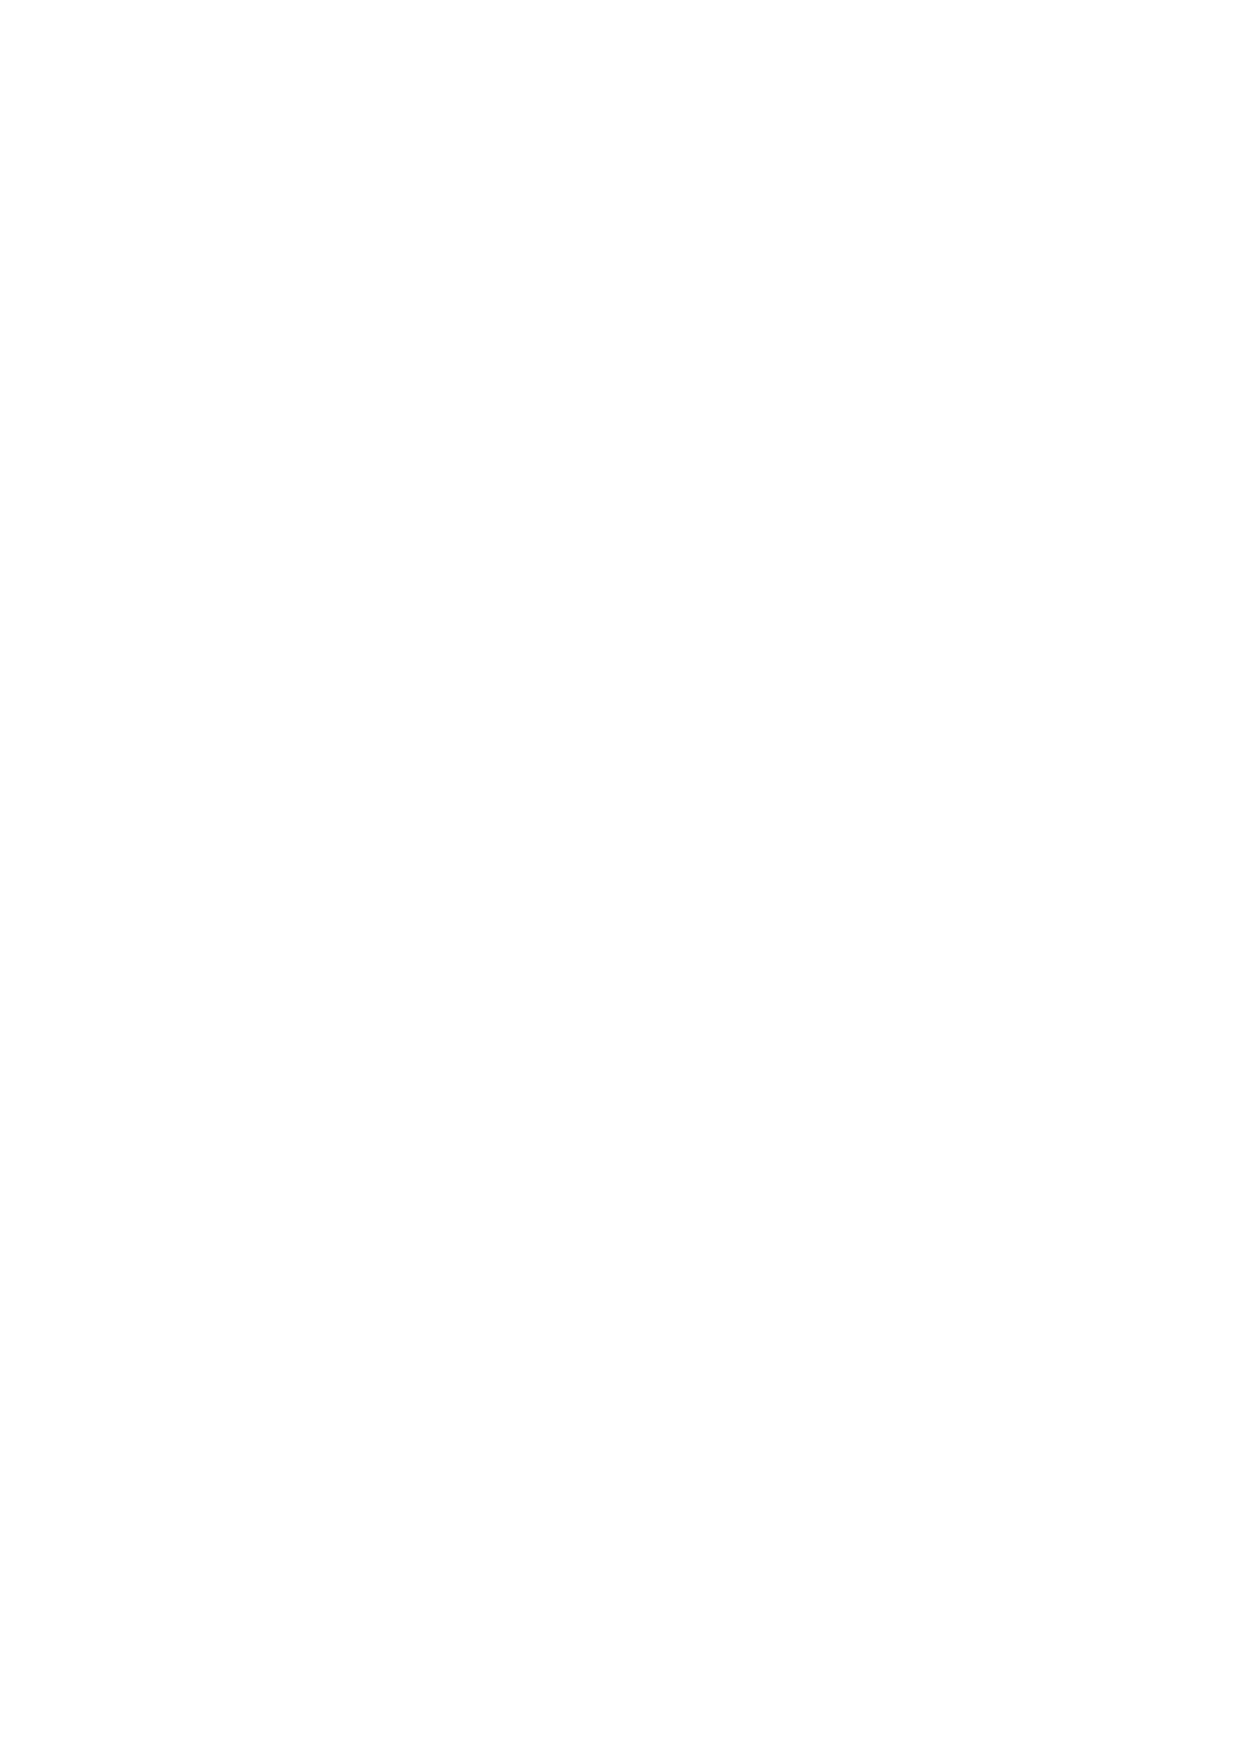
\includegraphics [scale=1]{jtr38}
	\caption{Transversal and non-transversal surfaces in the space.}
	\label{fig:3.8}
\end{figure}

The following fundamental theorem follows from Thom.\footnote{Thom's Transcendence Theorem, as well as its generalization given below, were an important part of his Catastrophe theory. This theory includes, in part, the theory of peculiarity of mappings and functions as well as the theories of bifurcation of dynamic systems.

It is worth adding that, in the case of the generalization of Thom's Theorem on the case of non-compact manifolds, special topologies (so called Whitney topologies) are introduced in the $C^k$ class projection space.}

\begin{theorem}\emph{(Thom).}\label{theo:3.6}
	Let $M$, $A$ and $B$ be fixed compact manifolds as above. Then the set of maps $f:A\longmapsto M$ that are transversal to $B$ is open and dense in $C^r (A,M)$.
	
	This means that, on the one hand, if the mapping $f_0$ is transversal to $B$, then any mapping $f_{\varepsilon}$ is transversal to $B$, and, on the other hand, if $f_0$ is not transversal,  then there exists a map $f_{\varepsilon}$ arbitrarily close to it that is already transversal to $B$ .
	
	\begin{proof}
		It is easy to see that we can limit ourselves to the local situation when $A\subset \mathbb{R}^{m}$ and $M\subset \mathbb{R}^{n}$ are open subsets and
		$$
		B=\left\{ y_{1}=\ldots =y_{n-k}=0\right\} \cap M
		$$
		is (locally) a subspace of codimension $n-k$ (Task 3.16).
		
		Then $f(x)=\left( f_{1}(x),\ldots f_{n}(x)\right) $ and
		$$
		T_{y}B=\left\{ q\in \mathbb{R}^{n}:q_{1}=\ldots =q_{n-k}=0\right\} \subset
		T_{y}M=\mathbb{R}^{n}.
		$$
		If $f(x_{0})\in B$, i.e., $f_{1}(x_{0})=\ldots f_{n-k}(x_{0})=0$, then $f$ is transversal at $x_0$ to $B$ if and only if the vectors $f_{\ast }\partial _{x_{1}},\ldots ,f_{\ast }\partial _{x_{m}}$ together with the vectors $\partial _{yn-k+1},\ldots \partial _{y_{n}}$ expand $\mathbb{R}^{n}$. (Here $\partial _{x_{j}}$ and $\partial _{y_{k}}$ are the base vectors in $\mathbb{R}^{m}$ and $\mathbb{R}^{n}$ respectively.) In addition, the projections of the $f_{\ast }\partial _{x_{j}}$ vectors on the quotient space $T_{y}M/T_{y}B\simeq \mathbb{R}^{n-k}$ expand the space. This means that matrix$$
		C=
		\begin{pmatrix}
		\partial f_{1}/\partial x_{1} & \ldots  & \partial f_{1}/\partial x_{m} \\
		\vdots  & \ddots  & \vdots  \\
		\partial f_{n-k}/\partial x_{1} & \ldots  & \partial f_{n-k}/\partial x_{m}%
		\end{pmatrix}
		$$
		has rank $\textrm{rk\,}C\geq n-k$.
		
		We have two possibilities:
		\begin{enumerate}[(i)]
			\item $m<n-k$ and then the rank is smaller than $n-k$, which is impossible,
			\item $m\geq n-k$ (then the property of \textrm{rk} $C\geq n-k$ is an open condition in the matrix space).
		\end{enumerate}
	In the case (i) transversality means that there is no $f (A)$ in $B$ and that it is an open condition in the mapping space. Also in case (ii) it is not difficult to show that the condition of transversality is open (Task 3.13).
	
	To prove the inherent nature of transversality we need to introduce additional concepts (Task 3.14).
	
	In case (ii) let us consider the local mapping $g:A\longmapsto R^{n-k},$%
	$$
	g(x)=(f_{1}(x),\ldots ,f_{n-k}(x)).
	$$	
	Recall (see Definition \ref{def:3.7} below), where $x_0$ is the critical point for $g$ if rk$\frac{\partial g}{\partial x}(x_{0}) = $ rk$C<n-k,$ and the value $g (x_0)$ is called the critical value for $g$. We will use the classical Sard Theorem (Theorem \ref{theo:3.8} below), which ensures that the set of critical values for $g$ is `rare'. According to Task 3.15 $f\pitchfork B$ iff 0 is not a critical value for $g$. Let $z$ be a non-critical value for $g$ and close to zero. We will distort the mapping $f=(g,h)$ in the following way
	$$
	f_{\varepsilon }(x)=(g(x)-z,h(x)).
	$$
	It is easy to see that $f_{\varepsilon }$ is transversal to $B$ (Task 3.16).
	\end{proof}
\end{theorem}

\begin{definition}\label{def:3.7}
	Let $h:\mathbb{R}^{m}\longmapsto \mathbb{R}^{l}$ be a differentiable mapping. We say that $x_0$ is a \textbf{critical point} for $h$ if rk $\frac{\partial h}{\partial x}(x_{0})$ is not maximal. The value $h(x_0)$ at the critical point is called the \textbf{critical value} for $h$.
\end{definition}

\begin{theorem}\emph{(Sard).}\label{theo:3.8}
	The set of critical values for the differential mapping $h:\mathbb{R}^{m}\longmapsto \mathbb{R}^{l}$ of a sufficiently high class of smoothness has zero Lebesgue measure.
	\begin{proof}[Idea of the proof]
		Consider the case of $m = l = 1$. It is not excluded that the critical values for $g$ can form a set of gestures in $\mathbb{R}$. We can, however, cover every critical point $x_j$ with a section $I_{j}$ of width $\left\vert I_{j}\right\vert \leq \varepsilon $ for any small $\varepsilon $. Since $g^{\prime }(x_{j})=0,$ then the length of the image $g(I_{j})$ of that segment will be the width of the order $ O(\varepsilon ^{2})=O(\varepsilon )\left\vert I_{j}\right\vert $ (see Figure \ref{fig:3.9}). Therefore,
		$$
		\left\vert g\left( \bigcup I_{j}\right) \right\vert \leq O(\varepsilon
		)\cdot \left\vert \bigcup I_{j}\right\vert \leq O(\varepsilon ),
		$$
		tends to zero as $\varepsilon \rightarrow 0.$
		
		The same argument applies to any $m\leq l $ (Task 3.17). When $m>l$ proof is more complicated (with the division of $\mathbb{R}^{m}$ into subsets of the constant order of the matrix $\partial h/\partial x$).
		\begin{figure}[!ht]
			\centering
			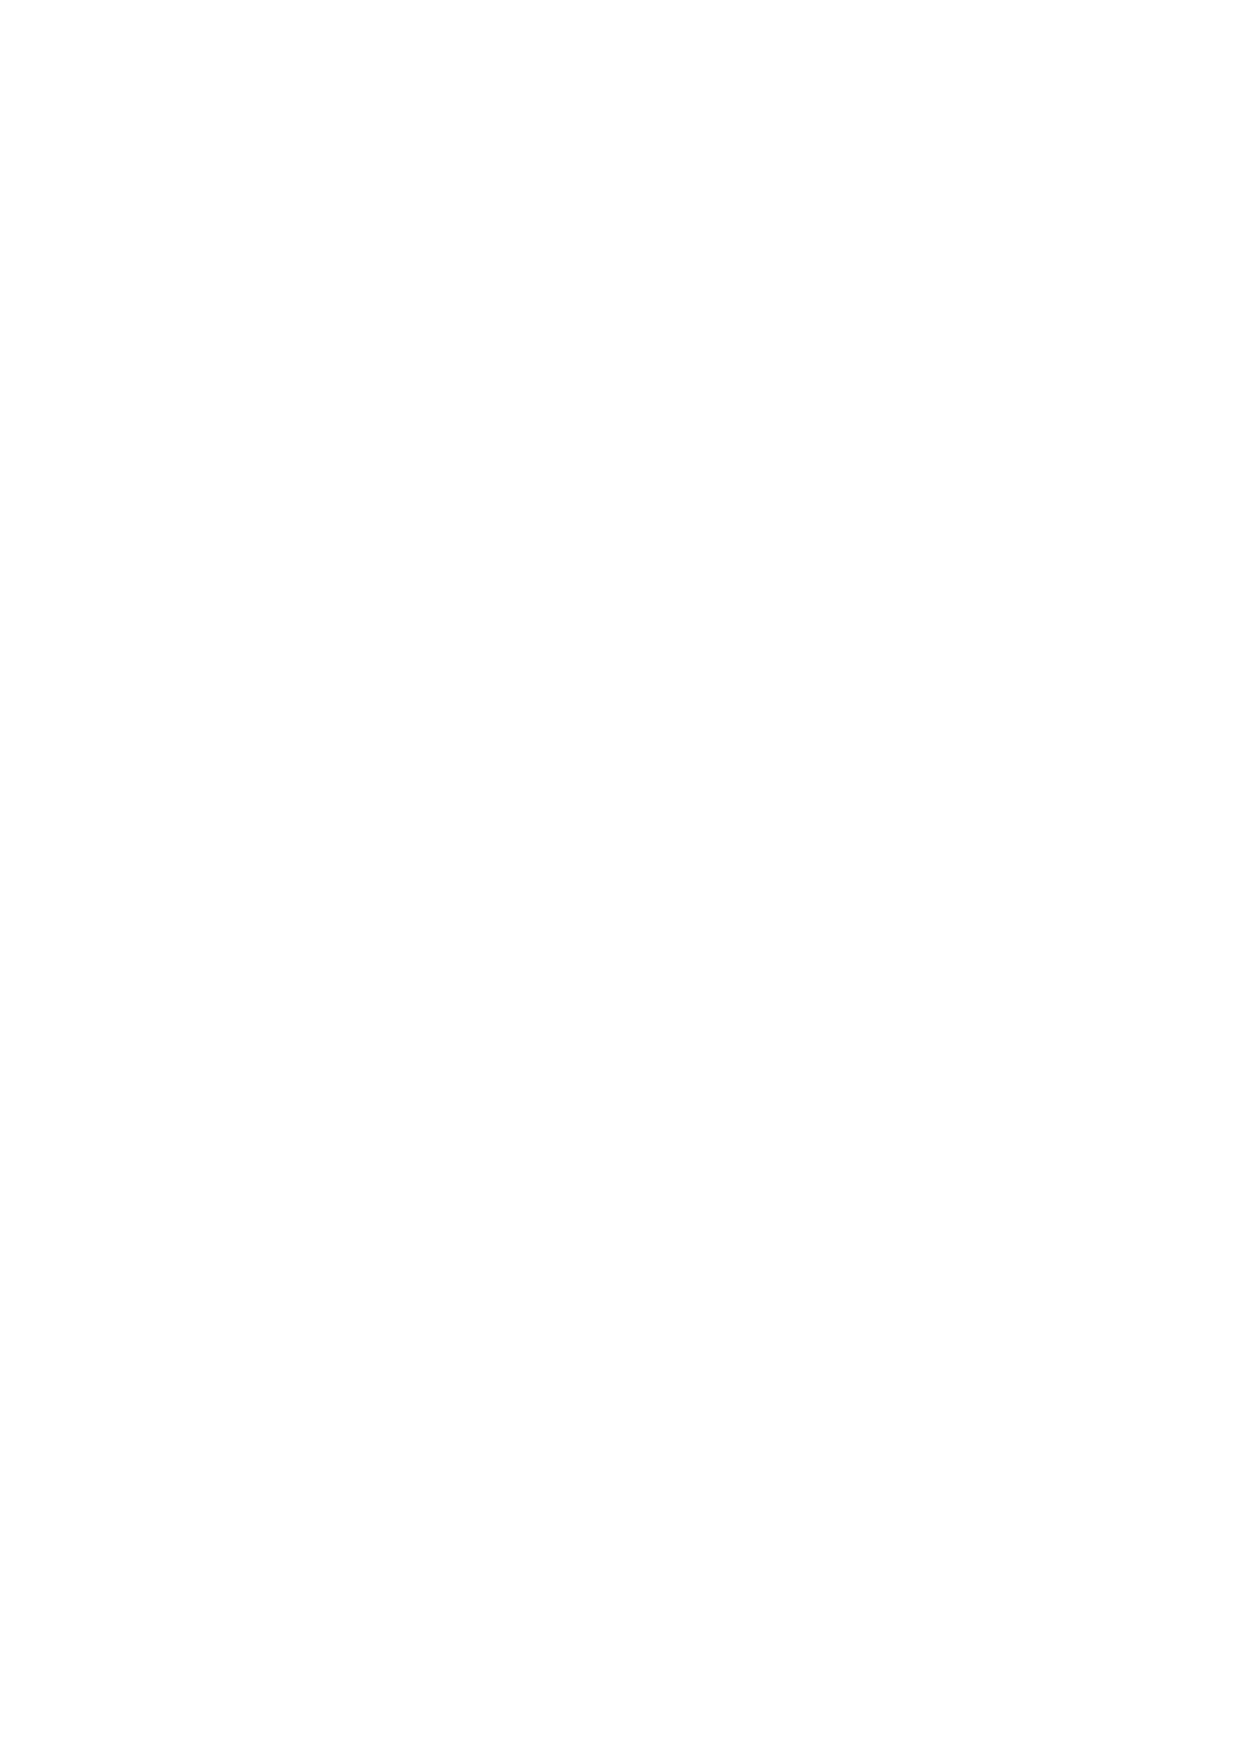
\includegraphics [scale=1.3]{jtr39}
			\caption{Sard Theorem.}
			\label{fig:3.9}
		\end{figure}
	\end{proof}
\end{theorem}

The following definition is needed to generalize Thom's Theorem. Let
\begin{equation}
\label{3.3}
f:\mathbb{R}^{m}\longmapsto \mathbb{R}^{n}
\end{equation}
be a mapping sufficiently many times differentiable. With such mapping, we can associate a series of geometric objects. The first is the graph
$$
\left\{ (x,f(x))\right\} \subset \mathbb{R}^{m}\times \mathbb{R}^{n}=:J^{0}(\mathbb{R}^{m}, \mathbb{R}^{m}).
$$
Another graph of the derivative is the graph of the mapping $Df: x\longmapsto
(y,p) = (f(x), \frac{\partial f}{\partial x}(x))$,
$$
\left\{ \left( x,f(x),\frac{\partial f}{\partial x}(x)\right) \right\}
\subset \mathbb{R}^{m}\times \mathbb{R}^{n}\times \mathbb{R}^{m\cdot n}=:J^{1}(\mathbb{R}^{m},\mathbb{R}^{n}).
$$
In general, the graph of mapping of the $r$-th order mapping derivative $x \longmapsto (f(x), Df(x),\linebreak \ldots, D^{r}f(x))$ is a subset (relatively large) of the space denoted by $J^{r}(\mathbb{R}^{m},\mathbb{R}^{n})$.

\begin{definition}
	The $J^{r}(\mathbb{R}^{m},\mathbb{R}^{n})$ spaces are called \textbf{jets spaces of  order $r$} from $\mathbb{R}^{m}$ to $\mathbb{R}^{n}.$ Every mapping of the form \eqref{3.3} is associated with his \textbf{$r$-th jet}
	$$
	x\longmapsto j^{r}f(x)=(x,f(x),Df(x),\ldots ,D^{r}f(x))\in J^{r}(\mathbb{R}%
	^{m},\mathbb{R}^{n}).
	$$
	Analogously, if $A$ and $M$ are manifolds of dimension $m$ and $n$ respectively, it defines the spaces $J^{r}(A,M)$ of the jets mapped from $A$ to $M$, and each different map $f:A\longmapsto M$ is bound to its $r-$th jet $j^{r}f:A\longmapsto J^{r}(A,M).$
\end{definition}

\begin{definition}
	If $C\subset J^{r}(A,M)$ is a submanifold, we say that the mapping $f:A\longmapsto M$ is \textbf{transversal to $C$} (denotation $f\pitchfork C$) when $j^{r}f\pitchfork C.$
\end{definition}

\begin{theorem}\emph{(Thom).} \label{theo:3.11}
	Let $A$, $M$ and $C\subset J^{r}(A,M)$ be fixed. Then the set of mappings $f:A\longmapsto M$, which are transversal to $C$, is open and dense in the set of all such mappings.
	\begin{proof}
		This proof in a large part repeats the proof of Theorem \ref{theo:3.6}. The basic difference lies in the proof of density, more specifically, in the choice of the perturbation. Instead of replacing $f(x)\rightarrow f(x)-z$ (where $z$ is a `small' noncritical value for $f$), it is replaced by $f(x)\rightarrow
		f(x)-z-\tilde{p}(x)-\tilde{q}(x,x)-\ldots -\tilde{s}(x,\ldots x),$ where $\tilde{p}$, $\tilde{q}$, $\ldots ,\tilde{s}$ are `small' linear transformations, homogeneous squares, or homogeneous degrees $r$.
	\end{proof}
\end{theorem}

\begin{example}\label{example:3.12}
	Certain natural conditions for mappings are interpreted as conditions for its transversality in jets. For example, the condition
	$$
	\frac{\partial f}{\partial \lambda }(x,\lambda )\cdot \frac{\partial ^{2}}{%
		\partial x^{2}}f(x,\lambda )\not=0\text{ \ where \ }f(x,\lambda )=\frac{%
		\partial f}{\partial x}(x,\lambda )=0
	$$
	follows from the simultaneous transversality of mapping
	$$
	j^{1}f:\mathbb{R}^{2}=\left\{ \left( x,\lambda \right) \right\} \longmapsto
	J^{1}(\mathbb{R}^{2},\mathbb{R})=\left\{ \left( x,\lambda
	,y,p_{x},p_{\lambda }\right) \right\}
	$$
	to the two submanifolds $$
	C_{1}=\left\{ y=0\right\} \text{ \ and \ }C_{2}=\left\{ y=p_{x}=0\right\} .
	$$
	Indeed, transversality to $C_{1}$ means that $\frac{\partial
	y}{\partial x}=\frac{\partial f}{\partial x}\not=0$ or $\frac{\partial y}{%
	\partial \lambda }=\frac{\partial f}{\partial \lambda }\not=0$ when $y=f(x,\lambda )=0.$
	Meanwhile, transversality to $C_{2}$ means that $\left\vert
	\begin{array}{ll}
	f_{x}^{\prime } & f_{\lambda }^{\prime } \\
	f_{xx}^{\prime \prime } & f_{x\lambda }^{\prime \prime }%
	\end{array}%
	\right\vert \not=0$ where $y=f=0$ and $p_{x}=f_{x}^{\prime }=0.$
\end{example}
\bigskip
In the problems of bifurcation theory always, when conditions of a similar character as in Example \ref{example:3.12} appear, we can assume that either are satisfied with probability 1 or with the same probability can not be satisfied. The second case occurs when $\dim A+\dim C<\dim J^{r}(A,M).$ This is a practical conclusion from Thoma's theorem.

\subsection*{Tasks}
\begin{task}
	In the case of $m\geq n-k$, note that (in the proof of Theorem \ref{theo:3.6}) rk$C\geq n-k$ means rk $C=n-k$. Use the Implicit Function Theorem to show that $f^{-1}(B)\subset A$ in a neighborhood of $x_{0}$ is a submanifold in $A$ of codimension $n - k$. Then show that for any $f_{\varepsilon }$ near to $f$, also $f_{\varepsilon }^{-1}(B)$ is a local submanifold of codimension $n-k$ close to $f^{-1}(B)$. In this case, deduce from the openness of a subset of the matrix of the order $n-k$ in the space of the matrices of dimension $(n-k)\times n$, that $f_{\varepsilon }$ is transversal to $B$ in the neighborhood of $x_0$.
\end{task}

\begin{task}
	Show the local duality of transversal property in the case of $m <n-k$.
	
	Tip: Select the appropriate disturbance $f_{\varepsilon }$ for $f$, which is not transversal to $B$.
\end{task}

\begin{task}
	Show that $f\pitchfork B$ if and only if 0 is not critical for the mapping $g$.
\end{task}

\begin{task}
	Complete the proof of Theorem \ref{theo:3.6}.
	
	Tip: Use the corresponding unity distribution $1=\sum \varphi _{j}(x)$ in $A$ associated with local affine maps in $A$, $M$ and $B$. Local disorder select in the form $f_{\varepsilon}=\left( g-\psi_{k}(x) z_{k}, h(x)\right)$, with the corresponding functions $\psi_{k}(x)$ with a compact support and `small' vectors $z_{k}$. Finally, take advantage of the compactness of $A$.
\end{task}

\begin{task}
	Prove the Sard Theorem for cases $m <l$ and $m = l> 1$.
\end{task}
\section{Codimension 1 bifurcations}\label{sec:3.3}

Bifurcations autonomous vector fields will be divided into local and non-local.

\textbf{Local bifurcation}s occur around the singular point $x = 0$ for the bifurcation parameter value. More precisely, we have a family
$$
\dot{x}=v(x;\mu )
$$%
such that
$$
v(x,0)=Ax+\ldots .
$$
In the case of typical 1-parameter families, the violation of the hyperbolic condition (i.e., $\textrm{Re}\lambda _{j}(A)\not=0$ for all the eigenvalues) occurs in two cases:
\begin{enumerate}
	\item $\lambda _{1}(A)=0$ and $\textrm{Re}\lambda _{j}(A)\not=0$ for $j>1$; this is a \textbf{saddle-node bifurcation}.
	\item $\lambda _{1}=\bar{\lambda}_{2}=i\omega \in i\mathbb{R}\setminus 0$
	and $\textrm{Re}\lambda _{j}\not=0$ for $j>2$; this is a \textbf{birth of the limit cycle bifurcation} or the \textbf{Andronov-Hopf bifurcation}.
\end{enumerate}

We have three \textbf{non-local bifurcations} associated with the periodic orbit $\gamma$ for the field $v (x, 0)$. Let $\lambda _{j}$ be the eigenvalues of part of the linear transformation of Poincaré's return. Recall that the hyperbolic condition for $\lambda _{j}$ denotes that $\left\vert \lambda _{j}\right\vert \not=1$ for all $j$. Thus, typical codimension 1 bifurcations may occur in the following cases:
\begin{enumerate}\setcounter{enumi}{2}
	\item $\lambda _{1}=1$ and $\left\vert \lambda _{j}\right\vert \not=1$
	for $j>1$; this is a \textbf{saddle-node bifurcation for periodic orbit}.
	\item $\lambda _{1}=-1$ and $\left\vert \lambda _{j}\right\vert \not=1$
	for $j>1$; this is a \textbf{period doubling bifurcation}.
	\item $\lambda _{1}=\bar{\lambda}_{2}\in \mathbb{S}^{1}\setminus
	\{1,-1\}$. Here the cases where $\lambda _{1}=e^{2\pi ik/m}$ is an element of degree $m=1$, they are called \textbf{resonances}; in addition, when $m = 3, 4$ we are talking about a \textbf{strong resonance}.
\end{enumerate}

\begin{figure}[!ht]
	\centering
	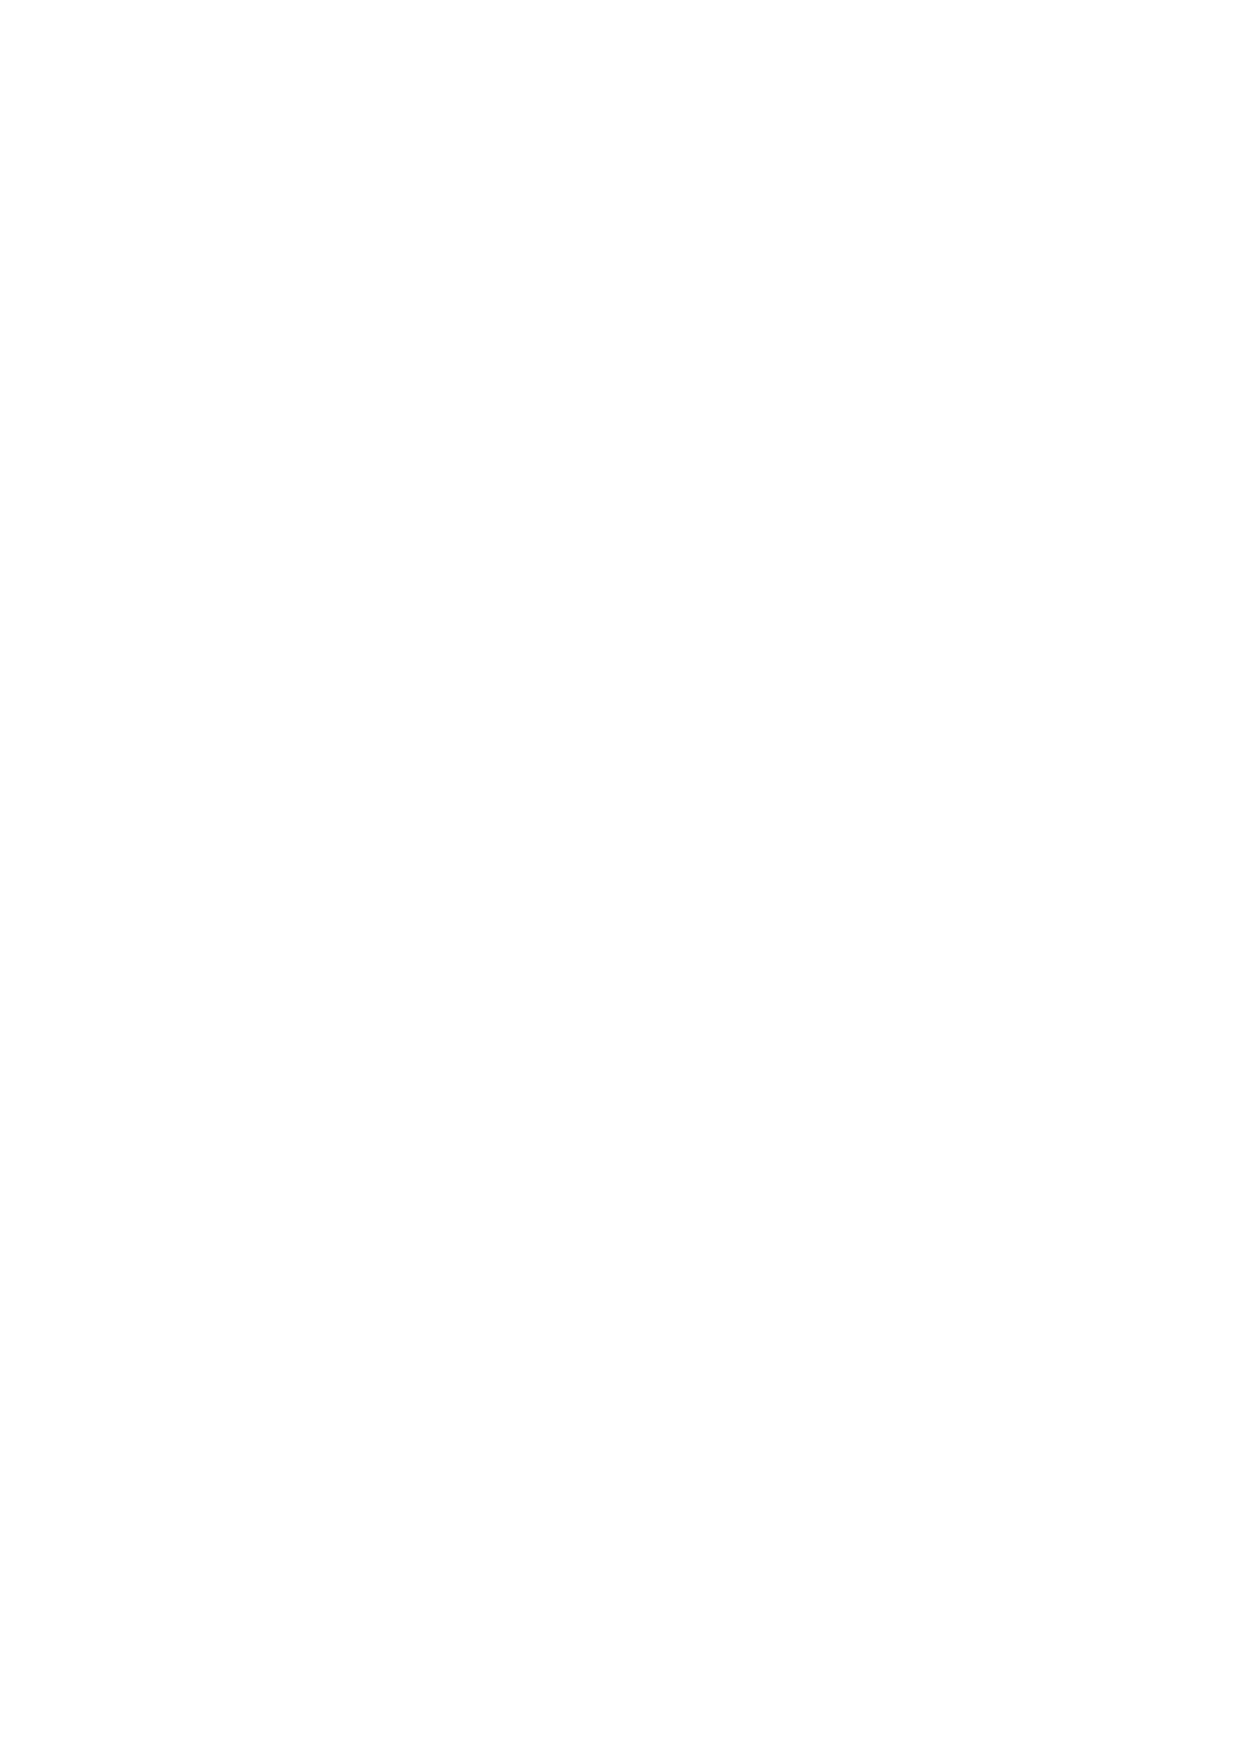
\includegraphics [scale=1.4]{jtr310}
	\caption{Connection separatrices and loop separatrices.}
	\label{fig:3.10}
\end{figure}

Finally, there are two \textbf{non-local bifurcations} related with the connection separatrices (see Figure \ref{fig:3.10}):
\begin{enumerate}\setcounter{enumi}{5}
	\item \textbf{Separatrix connection} between different saddles.
	\item \textbf{Separatrix loop} of one saddle.
\end{enumerate}

\subsection{Reduction to center manifold and Poincaré-Dulac normal form} \label{subsec:3.3.1}

Let's assume we have the vector field
$$
\dot{x}=v(x)=Ax+\ldots
$$
with the singular point $x = 0$. We can assume that matrix $A$ has diagonal blocks
\begin{equation}
\label{3.4}
A=A^{s}\oplus A^{u}\oplus A^{c},
\end{equation}
where $A^s$ (respectively $A^{u}$ and $A^{c}$) has eigenvalues with $\textrm{Re}\lambda _{j}<0$ (respectively with $\textrm{Re}\lambda _{j}>0$ and with $\textrm{Re}\lambda _{j}=0).$

\begin{theorem}\emph{(Shoshitaishvili).} \label{theo:3.18}
	In the situation above, there is a local homeomorphism $h:\left( \mathbb{R}^{n},0\right) \longmapsto \left( \mathbb{R}^{n},0\right) $ performing a phase portrait of field $v(x)$ for the phase portrait of the following field
	\begin{equation}
	\label{3.5}
	\dot{y}_{1}=-y_{1},\text{ \ }\dot{y}_{2}=y_{2},\text{ \ }\dot{y}%
	_{3}=w(y_{3}),
	\end{equation}
	where
	$$
	w(y_{3})=A^{c}y_{3}+\ldots
	$$
\end{theorem}

The proof of this theorem is technical and complex (see \cite{Ar2}). Therefore, we will not quote it here. For this we will draw from it very practical applications. We also note that this theorem is a generalization of the Hartman-Grobman Theorem.

\begin{definition}
	The submanifold given by the equation
	$$
	W^{c}=\left\{ y_{1}=0,\text{ }y_{2}=0\right\}
	$$
	(in terms of \eqref{3.5}) is called \textbf{center manifold}.
\end{definition}

Shoshitaishvili Theorem says that in the case of non-hyperbolic singular point the `interesting part' of dynamics takes place on the central manifold.

For the family of vector fields $v(x,\mu )$ we can treat $\mu$ as an additional variable, i.e., we have the system
$$
\dot{x}=v(x,\mu ),\text{ \ }\dot{\mu}=0,
$$
to which we apply Theorem \ref{theo:3.18} (with $h(x,\mu )=(h_{0}(x,\mu ),\mu
$). We have the following \textbf{reductions to the center manifold}.

\begin{proposition}
	For the family $\dot{x}=v(x,\mu )$ with $v(x,0)=Ax+\ldots $, $A = A^{s}\oplus A^{u}\oplus A^{c}$, there is a local homeomorphism $(h_{0}(x,\mu ),\mu )$ giving the topological equivalent of this family to the following family
	$$
	\dot{z}=w(z,\mu ),\text{ \ }\dot{z}_{1}=-z_{1},\text{ \ }\dot{z}_{2}=z_{2}.
	$$
\end{proposition}

The very existence of the center manifold $W^{c}$ is a generalization of the Hadamard-Perron Theorem. It is possible to search for it as in Theorem \ref{theo:1.18}. In this case, the center manifold is not uniquely determined; it depends on the choice of field extension (or diffeomorphism) for all $\mathbb{R}^n$.

But there is a way to designate $W^c$ in a formal way. We look at it as a graph
$$
W^{c}=\left\{ x_{1}=f(x_{3}),\text{ \ }x_{2}=g(x_{3}):x_{3}\in E^{c}\right\}
$$
(where the coordinates $(x_1, x_2, x_3)$ are related to the decomposition \eqref{3.4}), which is invariant relative to the field $v (x)$. It turns out that the mappings $f:E^{c}\longmapsto E^{s}$ and $g:E^{c}\longmapsto E^{u}$ have unambiguously defined Taylor series at $x_3 = 0$, $f(x_{3}),g(x_{3})=O(\left\vert x_{3}\right\vert ^{2}).$ On $W^{c}$, which is the parameter called by $x_{3}\in E^{c},$ we obtain the vector field
$$
\dot{x}_{3}=w(x_{3}).
$$
This reduction to $ W ^ {c} $ is called \textbf{Lyapunov-Schmidt reduction}.

Unfortunately, it generally turns out that the dealing series of $f$ and $g$ are divergent (even if $v (x)$ is analytic). This also explains the ambiguity of the $W^c$ in a topological sense.

\begin{example} (Euler).
	Let's consider the system
	$$
	\dot{x}=x^{2},\text{ \ }\dot{y}=y-x^{2}.
	$$
	Here $ W ^ {u} = \left \{x = 0 \right \} $ is an unstable manifold. We are looking for a central manifold $W^{c}=\left\{ y= a_1 x + a_{2}x^{2}+a_{3}x^{3}+\ldots \right\} .$ By putting such $y$ into the system, we get
		$$
		\left( a_1 x +a_{2}x^{2}+a_{3}x^{3}+\ldots \right) -x^{2}=\left( a_1 +
		2a_{2}x+3a_{3}x^{2}+\ldots \right) x^{2}.
		$$
		This leads to the following recursion:  $a_1 = 0$ and $a_{2}=1$, $a_{n+1}=na_{n}$, with solution $a_{n}=(n-1)!.$ Thus, the central manifold is given by the unambiguous, but divergent, series
		$$
		y=\sum_{n\geq 2}(n-1)!x^{n}
		$$
		(Tasks 3.27 and 3.28).
\end{example}

Another tool useful in bifurcation theory, which also relies on (often divergent) formal series, is the next theorem. We consider the germs of analytical vector fields
\begin{equation}
\label{3.6}
\dot{x}=Ax+O(\left\vert x\right\vert ^{2}),\text{ \ \ }x\in \left( \mathbb{C}%
^{n},0\right) ,
\end{equation}
such that, the matrix $A$ is diagonal, $A=\textrm{diag}\left( \lambda
_{1},\ldots ,\lambda _{n}\right) .$ Let's recall the standard basis $ \left (e_ {1}, \ldots, e_ {n} \right) $ of $\mathbb{C}^{n}$ (therefore $x=\sum x_{j}e_{j}$), $x^{k}=x_{1}^{k_{1}}\ldots x_{n}^{k_{n}}$ and $\left\vert k\right\vert =k_{1}+\ldots +k_{n}.$

\begin{definition}
	We say that the eigenvalues satisfy the \textbf{resonance relation of type $\left( j,k\right)$}, $j\in	\{1,\ldots ,n\}$, $k=\left( k_{1},\ldots, k_{n}\right) \in \mathbb{N}^{n}$, if
	$$
	\lambda _{j}=k_{1}\lambda _{1}+\ldots k_{n}\lambda _{n}=(k,\lambda ).
	$$
\end{definition}

\begin{theorem}\emph{(Poincaré–Dulac).} \label{theo:3.23}
	Let's assume that we have the conjugated germ of the analytical vector field \eqref{3.6}. Then there is a formal change
	$$
	x=y+O(\left\vert y\right\vert ^{2})
	$$
	such that every component on the right is a formal power series in $y$, which leads to the system
	\begin{equation}
	\label{3.7}
	\dot{y}_{j}=\lambda _{j}y_{j}+\sum c_{j;k}y^{k},\text{ \ \ \ }j=1,\ldots ,n,
	\end{equation}
	where the sum on the right side of equation \eqref{3.7} runs at such polynomials $k=(k_{1},\ldots ,k_{n})$ such that the resonance relation of type $\left( j,k\right)$ is fulfilled.
	\begin{proof}
		Derivation into the \textbf{Poincaré-Dulac normal form} \eqref{3.7} takes place with the help of an alternation series of the form
		\begin{equation}
		\label{3.8}
		x=y+\sum_{j,k:\left\vert k\right\vert =m}b_{j,k}y^{k}e_{j},
		\end{equation}
		which adds homogeneous terms of the degree $ m$. (We start with $m = 2$, then we take $m = 3$, etc.) It is easy to see that the inverse of \eqref{3.8} has the form $y=x-\sum_{j,k:\left\vert k\right\vert
			=m}b_{j,k}y^{k}e_{j}+\ldots $\ (Task 3.29).
		
		Let us assume that only the resonant terms are present in the field \eqref{3.6} of degree $m-1$ (inductive assumption).  We want by substituting \eqref{3.8} to eliminate the non-resonant terms of degree exactly $m$. We have
		\begin{equation}
		\label{3.9}
		\dot{x}_{i}=\dot{y}_{i}+\sum_{k:\left\vert k\right\vert =m}b_{i,k}\left(
		y^{k}\right) ^{\cdot },
		\end{equation}%
		where
		$$
		\dot{y}_{i}=\lambda _{i}y_{i}+\left( \text{resonate terms of degree }\leq m\right)
		+h.o.t.
		$$%
		and
		$$
		\sum_{k:\left\vert k\right\vert =m}b_{i,k}\left( y^{k}\right) ^{\cdot }=\sum
		b_{i,k}\cdot \left( \lambda ,k\right) y^{k}+h.o.t.
		$$
		On the left side of the equation \eqref{3.9}, after substituting \eqref{3.8}, we have
		\begin{eqnarray*}
			\dot{x}_{i} &=&\lambda _{i}\left( y_{i}+\sum_{k:\left\vert k\right\vert
				=m}b_{i,k}y^{k}\right) +\left( \text{resonant terms of degree }\leq m-1\right) \\
			&&+\sum_{k:\left\vert k\right\vert =m}a_{i,k}y^{k}+h.o.t.
		\end{eqnarray*}
	Now, comparing the homogeneous terms of degree $m$, we get the equation$$
	b_{i,k}\cdot \left\{ (\lambda ,k)-\lambda _{i}\right\} =a_{i,k}.
	$$
	It is clear from this that if $\left( \lambda ,k\right) -\lambda _{i}\not=0$, then one can compute $b_{i,k}$ so as to eliminate the corresponding non-resonant term $x^{k}e_{i}$. Only resonant terms remain.
	\end{proof}
\end{theorem}

\begin{example}
	Let's consider the resonance node
	$$
	\dot{x}_{1}=x_{1}+\ldots ,\text{ \ \ }\dot{x}_{2}=nx_{2}+\ldots ,
	$$
	i.e., for $\lambda _{1}=1$ and $\lambda _{2}=n\in \mathbb{N}\setminus 1$. As we can see, the only resonant relation is $\lambda
	_{2}=n\lambda _{1}+0\cdot \lambda _{2}$. Thus, the Poincaré-Dulac normal form is
	$$
	\dot{y}_{1}=y_{1},\text{ \ \ }\dot{y}_{2}=ny_{2}+cy_{1}^{n}
	$$%
	(Task 3.30). It turns out that in this case the replacement leading to the normal form is analytical (if the germ was analytical).\footnote{In this case you can also count on situations where $n = 1$, that is, when the linear part is not diagonal. There is a natural extension of Theorem \ref{theo:3.23} to the case where the linear part of the field has non-trivial Jordan boxes.}
\end{example}

\begin{example}
	For the saddle-node
	$$
	\dot{x}_{1}=\ldots ,\text{ \ \ }\dot{x}_{2}=x_{2}+\ldots ,
	$$
	i.e., with $\lambda _{1}=0$ and $\lambda _{2}=1$, the resonance relations are of the form $\lambda _{1}=k\lambda _{1}+0\cdot \lambda _{2}$ and $\lambda
	_{2}=k\lambda _{1}+1\cdot \lambda _{2}$. Hence, the following Poincaré-Dulac form
	$$
	\dot{y}_{1}=\sum_{k\geq 2}a_{k}y_{1}^{k},\text{ \ \ }\dot{y}_{2}=y_{2}\left(
	1+\sum_{k\geq 1}b_{k}y_{1}^{k}\right) .
	$$
	It turns out that this normal form is not analytical at all.
\end{example}

\begin{example}\label{example:3.26}
	For the resonant saddle $(1: -1)$
	$$
	\dot{x}_{1}=x_{1}+\ldots ,\text{ \ \ }\dot{x}_{2}=-x_{2}+\ldots ,
	$$
	i.e., with $\lambda _{1}=1$ and $\lambda _{2}=-1$ , the resonance relations are of the form $\lambda _{1}=(k+1)\lambda _{1}+k\lambda _{2}$ and $\lambda
	_{2}=k\lambda _{1}+(k+1)\lambda _{2}.$ Hence, the following Poincaré-Dulac normal form
	$$
	\dot{y}_{1}=y_{1}\left( 1+\sum a_{k}\left( y_{1}y_{2}\right) ^{k}\right) ,\text{ \ \ }\dot{y}_{2}=-y_{2}\left( 1+\sum b_{k}\left( y_{1}y_{2}\right)
	^{k}\right).
	$$
	Also, this form is not general analytical (Task 3.31).
\end{example}

\subsection*{Tasks}
\begin{task}
	Find the central manifold of point $(0, 0)$ for the system from Task 1.33 at $a = -1$, i.e. for $\dot{x}=-x+y+x^{2}$, $\dot{y}=x-y+y^{2}$.
\end{task}

\begin{task}
	Find the approximation of the central manifold with the exactness to the cubic terms for the point $(0, 0, 0)$ of the system $\dot{x}=-y+x^{2}+zy$, $\dot{y} = x+xy+z^{2}$, $\dot{z}=z+xy$.
\end{task}

\begin{task}
	Show that the inverse transformation to the transformation \eqref{3.8} has the form as in the proof of Theorem \ref{theo:3.23}.
\end{task}

\begin{task}
	Show that in any other case of the node, i.e. when $1<\lambda _{2}/\lambda _{1}\not\in \mathbb{N}$, the normal Poincaré-Dulac form is linear (no non-linear resonant terms).
\end{task}

\begin{task}
	Generalize Example \ref{example:3.26} for the case $\left(p:-q\right)$ - resonant saddle, i.e. when $0<\lambda _{1}/\lambda_{2} = -p/q \in \mathbb{Q}$ (reduced fraction).
\end{task}

\subsection{Saddle-node bifurcation}
We have a 1-parameter family of vector fields
$$
\dot{x}=v(x;\mu )=v_{\mu }(x),\text{ \ \ }\left( x,\mu \right) \in \left(
\mathbb{R}^{n}\times \mathbb{R},0\times 0\right) .
$$
We apply the following conditions:
\begin{enumerate}
	\item $v(0;0)=0$, therefore $v(x;0)=Ax+\ldots $
	\item Matrix $A$ has one zero eigenvalue, $\lambda _{1}=0$, (in particular $\det A = 0$) and $\textrm{Re}\lambda_{j}\not=0$ for $j>1.$ Thus, it can be assumed that $A$ has the block form
	$$
	A=
	\begin{pmatrix}
	0 & 0 \\
	0 & B%
	\end{pmatrix}.
	$$
	\item Let $(x, y)$ be the linear coordinate system of the above form $A$. We can rewrite the system as
	$$
	\dot{x}=f(x,y;\mu ),\text{ \ \ }\dot{y}=By+\ldots ,
	$$
	where $f(0,0;0)=0$ and $f_{x}^{\prime }(0,0;0)=0.$ The next assumption is that
	$$
	\frac{\partial ^{2}f}{\partial x^{2}}(0,0;0)\not=0.
	$$
	\item The last assumption is that
	$$
	\frac{\partial f}{\partial \mu }(0,0;0)\not=0
	$$%
	(Task 3.34).
\end{enumerate}

\begin{remark}
	The above conditions are conditions in the space $J^{2}=J^{2}(\mathbb{R}^{n}\times \mathbb{R},\mathbb{R}^{n})$ of the kernels of order 2. These are conditions for transversality over certain submanifolds in $J^2$. By Theorem \ref{theo:3.11}, the typical $v (x; \mu)$ satisfies these conditions (see also Example \ref{example:3.12}).
\end{remark}

\begin{figure}[!ht]
	\centering
	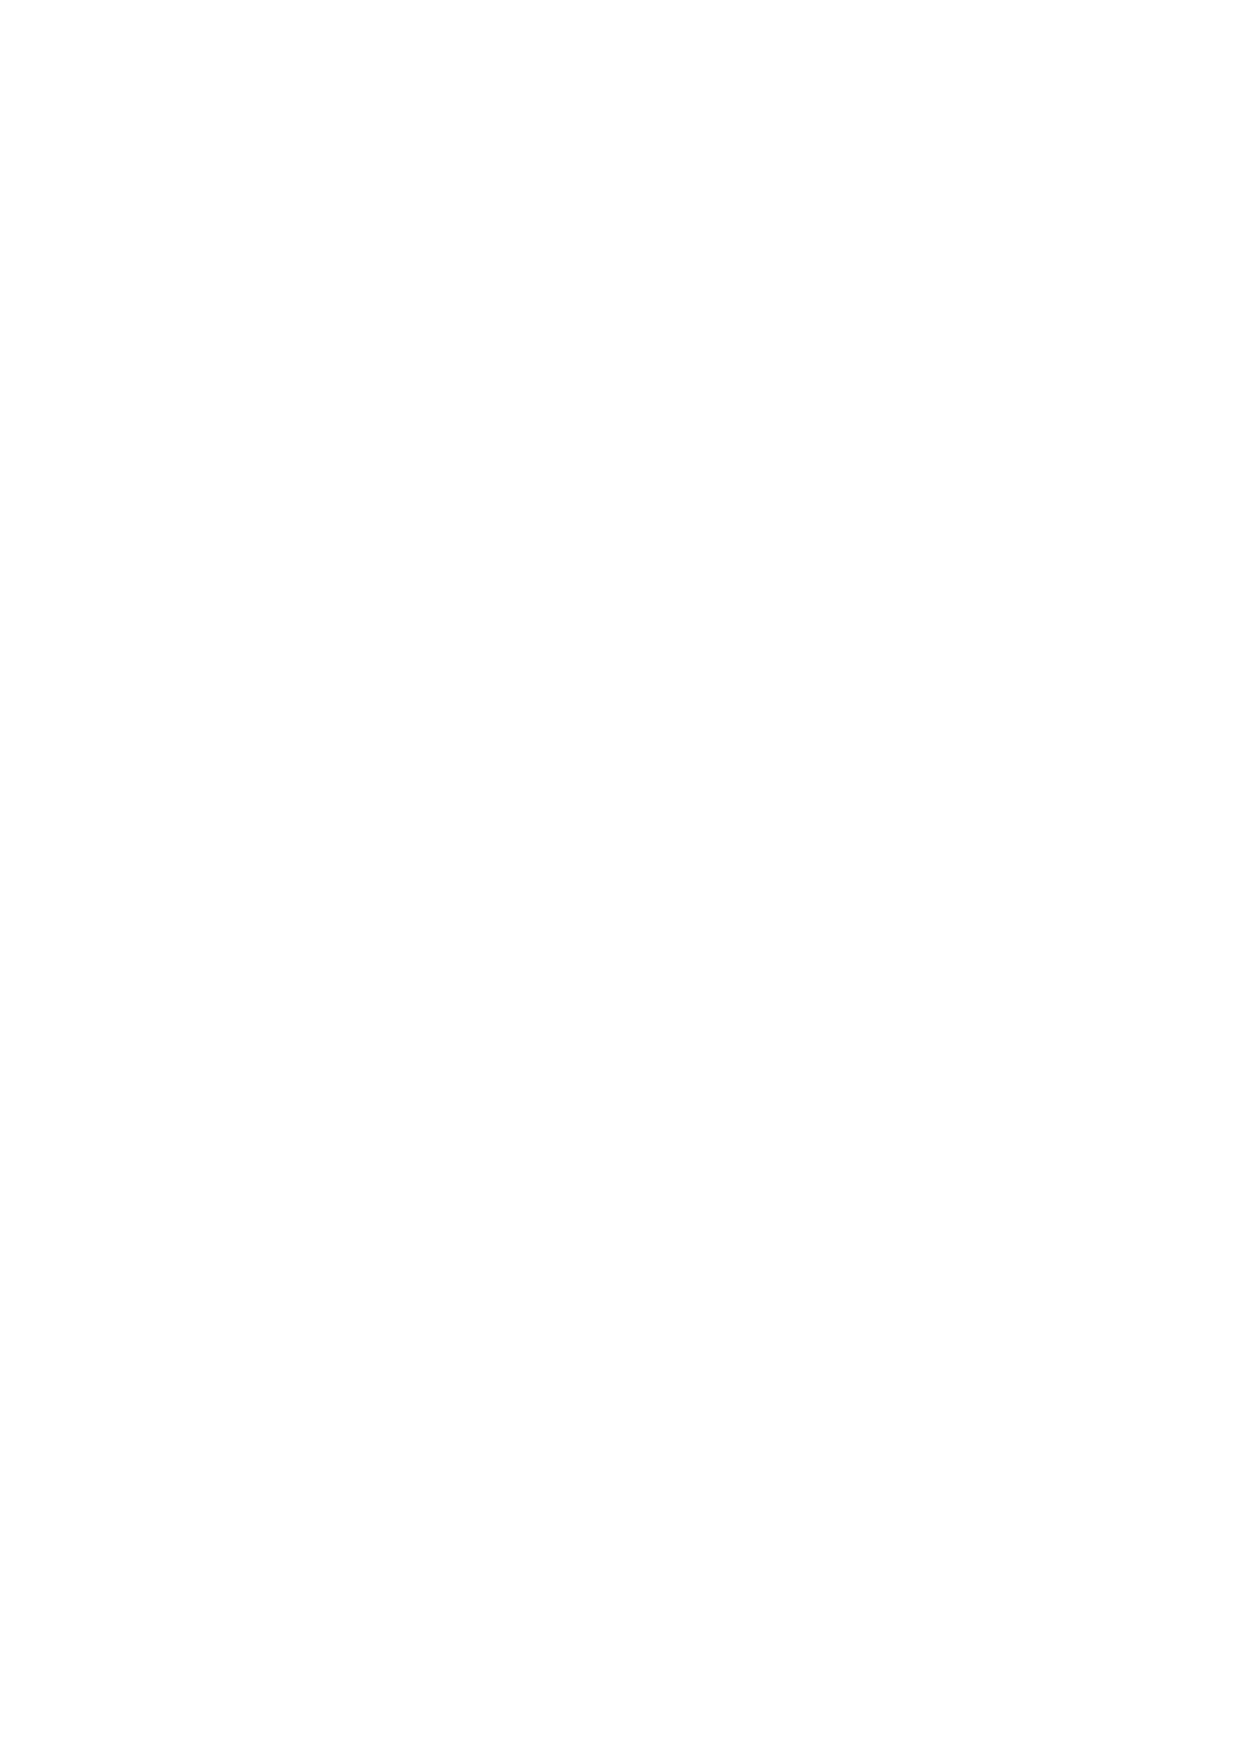
\includegraphics [scale=1]{jtr311}
	\caption{Saddle-node bifurcation.}
	\label{fig:3.11}
\end{figure}

\begin{theorem}
	If the above conditions are true, then the family $\left\{ v_{\mu }\right\} $ is versal. In particular, it is equivalent to one of the families of the form
	$$
	\dot{x}=\lambda \pm x^{2},\text{ \ \ }\dot{y}_{1}=-y_{1},\text{ \ \ } \dot{y}_{2}=y_{2}.
	$$
	
	\begin{proof}
		From the reduction theorem to the central manifold we can assume that we have a system of the form
		$$
		\dot{x}=f(x,\mu ),\text{ \ \ }\dot{y}_{1}=-y_{1},\text{ \ \ }\dot{y}_{2} = y_{2}.
		$$
		We have the following properties directly deriving from Conditions 1, 2, 3 and 4:
		\begin{enumerate}[(i)]
			\item $f(0,0)=0,$
			\item $f_{x}^{\prime }(0,0)=0,$
			\item $f_{xx}^{\prime \prime }(0,0)\not=0,$
			\item $f_{\mu }^{\prime }(0,0)\not=0.$
		\end{enumerate}
	Further proof is exactly as in Example \ref{example:3.3}.
	\end{proof}
\end{theorem}

Figure \ref{fig:3.11} shows the saddle-node bifurcation for a family of two-dimensional vector fields.

\subsection*{Tasks}
\begin{task}
	Show that Condition 4 has the following interpretations. From Condition 3 it follows that the equation $f_{x}^{\prime }=0$ has a unique solution $x=x_{0}(y,\mu )$ (local extreme point). Let $g(y,\mu )=f(x_{0}(y,\mu ),y;\mu )$ (value in this extreme). Then $\frac{\partial f}{\partial \mu }%
	(0,0;0)\not=0$\ $\Longleftrightarrow $\ $\frac{\partial g}{\partial \mu }%
	(0,0)\not=0.$
\end{task}

\begin{task}
	For a 2-parameter family of 1-dimensional vector fields, $\dot{x}=\lambda _{1}+\lambda _{2}x+x^{3}$ (personality deformation of the saddle-node type of the codimension 2) examine the bifurcation equilibrium point.
\end{task}

\subsection{Andronov-Hopf bifurcation}
We have a 1-parameter family of vector fields
$$
\dot{x}=v(x;\mu )=v_{\mu }(x),\text{ \ \ }\left( x,\mu \right) \in \left(
\mathbb{R}^{n}\times \mathbb{R},0\times 0\right) .
$$
We apply the following conditions:
\begin{enumerate}
	\item $v(0;0)=0$, therefore $v(x;0)=Ax+\ldots $
	\item $\lambda _{1}=\bar{\lambda}_{2}=i\omega \in i\mathbb{R}\setminus 0$
	and $\textrm{Re}\lambda _{j}\not=0$ for $j>2.$ This implies $\det A\not=0$ and from the Implicit Function Theorem, the equation $v(x;\mu )=0$ has the solution $x=x_{0}(\mu ),$ which corresponds to the equilibrium point. Then we move this equilibrium point to the beginning of the coordinate system:
	$x\longmapsto x-x_{0}(\mu ).$ Now we have the system
	$$
	\dot{x}=A(\mu )x+\ldots .
	$$
	\item The next assumption is that
	$$
	\frac{\partial }{\partial \mu }\textrm{Re}\lambda _{1,2}(\mu )|_{\mu =0}\not=0.
	$$	
	\item The last assumption is based on the Poincaré-Dulac normal form for $\mu = 0$. In the complex domain we have $\lambda_{1}=-\lambda _{2}$ and according to Example \ref{example:3.26} the normal form assumes the form
	$$
	\dot{z}_{1}=i\omega z_{1}\left( 1+\sum a_{j}\left( z_{1}z_{2}\right)
	^{j}\right) ,\text{ \ \ }\dot{z}_{2}=-i\omega z_{2}\left( 1+\sum b_{j}\left(
	z_{1}z_{2}\right) ^{j}\right) ,
	$$
	where $z_{1,2}=x_{1}\pm \sqrt{-1}x_{2}+\ldots =y_{1}\pm iy_{2}$ are (formal) complex variables after limitation to the center manifold. Since the starting field is real, then $z_{2}=\bar{z}_{1}$ and the above equations are in opposition to each other. In real variables $y_{1}=x_{1}+\ldots $ and $y_{2}=x_{2}+\ldots $ we get the following \emph{Poincaré-Dulac normal form for the focus}
	\begin{eqnarray*}
		\dot{y}_{1} &=&y_{1}\left( c_{3}r^{2}+c_{5}r^{4}+\ldots \right) -\omega
		y_{2}\left( 1+d_{3}r^{2}+\ldots \right) , \\
		\dot{y}_{2} &=&\omega y_{1}\left( 1+d_{3}r^{2}+\ldots \right) +y_{2}\left(
		c_{3}r^{2}+c_{5}r^{4}+\ldots \right) ,
	\end{eqnarray*}
	where $r^{2}=y_{1}^{2}+y_{2}^{2}.$ Here $c_{3},c_{5},\ldots $ are the Lyapunov-Poincaré focal quantities of the Definition \ref{def:2.13} (Task 3.40).
\end{enumerate}

The last non-degenerated condition says that
$$
c_{3}\not=0.
$$

The following statement is also called the \textbf{Theorem of the birth of limit cycles} and is perhaps the most well-known theorem of the bifurcation theory.

\begin{theorem}\emph{(Andronov-Hopf).}\label{theo:3.36}
	If the above conditions are true, then the family $\left\{ v_{\mu }\right\} $ is versal. In particular, it is equivalent to the family
	$$
	\dot{x}_{1}=x_{1}(\lambda \pm r^{2})-\omega x_{2},\text{ \ \ }\dot{x}%
	_{2}=\omega x_{1}+x_{2}(\lambda \pm r^{2}),\text{ \ }\dot{y}_{1}=-y_{1},%
	\text{\ \ }\dot{y}_{2}=y_{2},
	$$
	or (equivalent and on the central manifold) to the family
	\begin{equation}
	\label{3.10}
	\dot{z}=(\lambda +i\omega )z\pm z\left\vert z\right\vert ^{2},\text{ \ \ \ }%
	z=x_{1}+ix_{2}\in \mathbb{C}\simeq \mathbb{R}^{2}.
	\end{equation}
\end{theorem}

\begin{figure}[!ht]
	\centering
	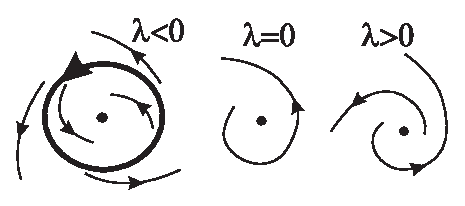
\includegraphics [scale=1.4]{jtr312}
	\caption{Unsafe loss of stability.}
	\label{fig:3.12}
\end{figure}

\begin{figure}[!ht]
	\centering
	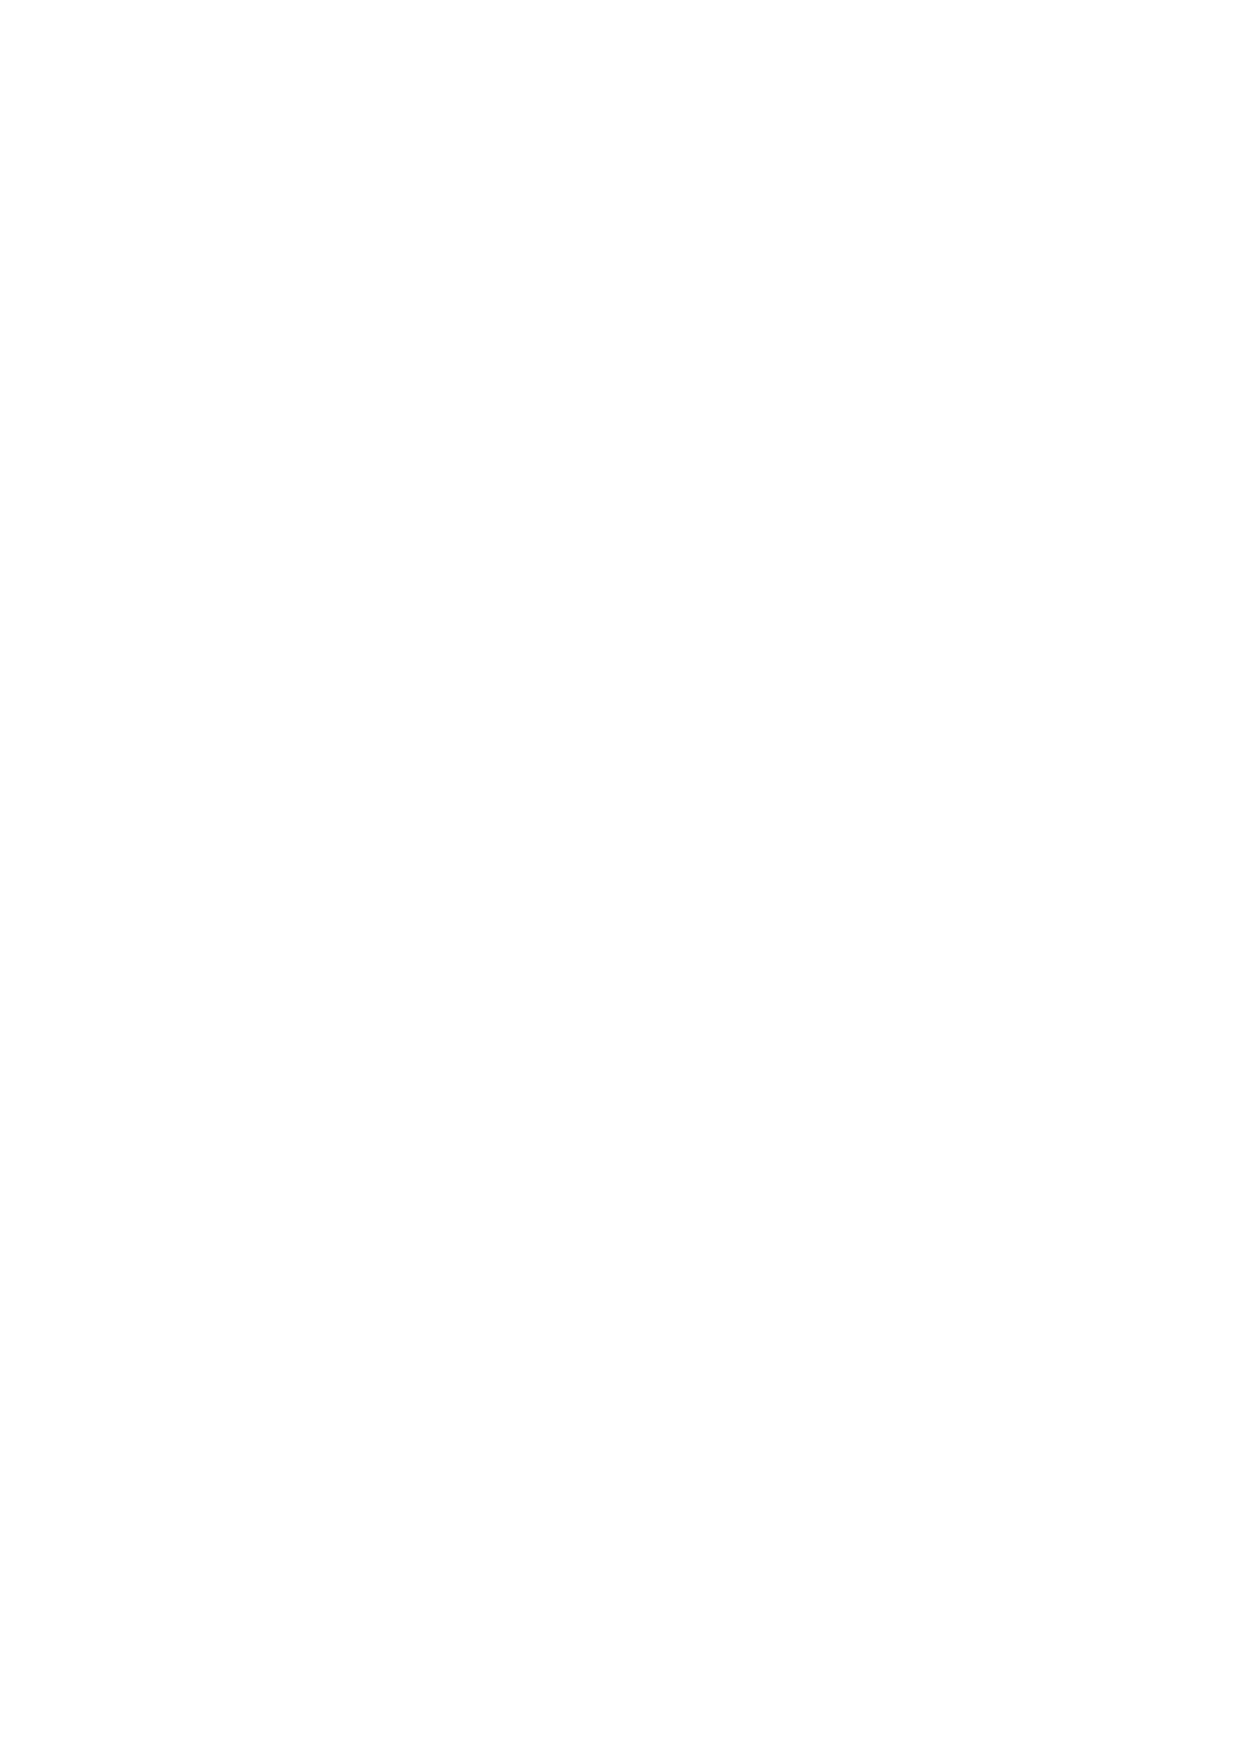
\includegraphics [scale=1.4]{jtr313}
	\caption{Safe loss of stability.}
	\label{fig:3.13}
\end{figure}

\begin{remark}
	To be able to change the orientation of the plane (e.g. $(x,y)\longmapsto (x,-y)$) we can assume that the frequency $\omega >0$. With this assumption we have two local bifurcations at \eqref{3.10} corresponding to two values $c_3 = 1$ and $c_3 = -1$. They are shown in Figures \ref{fig:3.12} and \ref{fig:3.13}, respectively. The difference between these drawings is of great practical importance.
	
	In Figure \ref{fig:3.12}, we observe the so-called \textbf{unsafe loss of stability}. Indeed, for $\lambda <0$, the equilibrium point is stable (although the `pool' of its attraction shrinks) and for $\lambda \geq 0$ the equilibrium point becomes `globally' unstable (here the system is completely fragmented).
	
	Figure \ref{fig:3.13} shows the so-called \textbf{safe loss of stability}. For $\lambda \leq 0$ the equilibrium point is `globally' stable and for $\lambda >0$ it loses stability. But for $\lambda >0$ there appears a stable limit cycle, located near the equilibrium point. So the system (e.g. mechanical) starts to oscillate slightly around the equilibrium position.
\end{remark}

\begin{proof}[Proof of Theorem \ref{theo:3.36}]
	As in the case of the Saddle-Node Bifurcation Theorem, we first reduce the question to a two-dimensional situation (on the center manifold).
	
	Adding to the proof of the Poincaré-Dulac Theorem to the next, we bring the whole family to the following normal form, modulo terms of order $\geq 4$:
	\begin{equation}
	\label{3.11}
	\dot{z}=\left( c_{1}(\mu )+i\omega (\mu )\right) z+(c_{3}(\mu )+id_{3}(\mu
	))\left\vert z\right\vert ^{2}z+O(\left\vert z\right\vert ^{4}),
	\end{equation}
	$z=y_{1}+iy_{2}$, where $c_{1}(0)=0$, $c_{1}^{\prime }(0)\not=0$ and $%
	c_{3}(0)\not=0$ (Task 3.41). We can easily assume that $c_{1}(\mu )=\mu $, and, going to the polar coordinate system, $z=re^{i\varphi }$, we can write
	\begin{equation}
	\label{3.12}
	\dot{r}=r\left( \mu +c_{3}r^{2}+O(r^{3})\right) ,\text{ \ \ }\dot{\varphi}%
	=\omega +O(r^{2})
	\end{equation}
	(Task 3.42).
	
	\begin{figure}[!ht]
		\centering
		\includegraphics [scale=1.4]{jtr314}
		\caption{Proof of Andronov-Hopf Theorem.}
		\label{fig:3.14}
	\end{figure}

	For the system \eqref{3.12}, we define the Poincaré's return map $P:\left\{ \varphi =0\right\}$
	$ \longmapsto \left\{ \varphi =2\pi \right\} $ as in Figure \ref{fig:3.14}. By rescaling, we can put $c_3 = \pm 1$. We assume that $c_3 = 1$. We divide the further analysis into three cases.
	\begin{enumerate}[(a)]
		\item For $\mu \geq 0$ we have $\dot{r}>0$ (for $r>0$),  that is $ P (r)> r $ and there are no limit cycles.
		\item Let $\mu <0$. Consider the area $\left\{ 0\leq r\leq 2\sqrt{%
			-\mu }\right\} $. Let's make the following normalization
		$$
		r=\tau R,\text{ \ \ }\mu =-\tau ^{2}.
		$$
		Then in the area $\left\{ 0\leq R\leq 2\right\}$ we get the system
		\begin{equation}
		\label{3.13}
		\dot{R}=\tau ^{2}R\left( -1+R^{2}+O(\tau )\right) ,\text{ \ \ }\dot{\varphi}%
		=\omega +O(\tau^2 )
		\end{equation}
		for the small parameter $\tau$. Now it's easy to calculate the Poincaré transformation. Let's notice that the solution of the system \eqref{3.13} with the initial condition $R(0)=R_{0}$, $\varphi (0)=0$
		meets $R(t)=R_{0}+O(\tau ).$ Therefore
		\begin{eqnarray*}
			P(R_{0})-R_{0} &=&\int_{0}^{2\pi }\frac{dR}{d\varphi }d\varphi =\frac{\tau
				^{2}}{\omega }\int_{0}^{2\pi }\frac{R(-1+R^{2}+O(\tau ) )}{1+O(\tau ) }d\varphi
			\\
			&=&\tau ^{2}\frac{2\pi }{\omega }R_{0}(R_{0}^{2}-1+O(\tau )).
		\end{eqnarray*}
		Let's denote $F(R_{0},\tau )=(P(R_{0})-R_{0})/\tau ^{2}=F_{0}(R_{0})+O(\tau )$, where the graph of function $F_{0}(R_{0})=\pi R_{0}(R_{0}^{2}-1)/\omega $ is shown in Figure \ref{fig:3.15}. We see that the equation $F(R_{0},\tau
		)=0$ has exactly two simple solutions $R_{0}=0$ and $R_{0}=1+O(\tau )$ (Task 3.43). The first of them corresponds to the equilibrium point and the second to the unstable limit cycle $\left\{ r=\sqrt{-\mu }\right\}$.
		\item For $\mu <0$, consider the area $\left\{ 2\sqrt{-\mu }%
		<r<\varepsilon \right\} $ for small $\varepsilon > 0$ (independent of $\mu$). From \eqref{3.12} it is easy to see that here $\dot{r}>0$ and there can be no limit cycles.
		
		\begin{figure}[!ht]
			\centering
			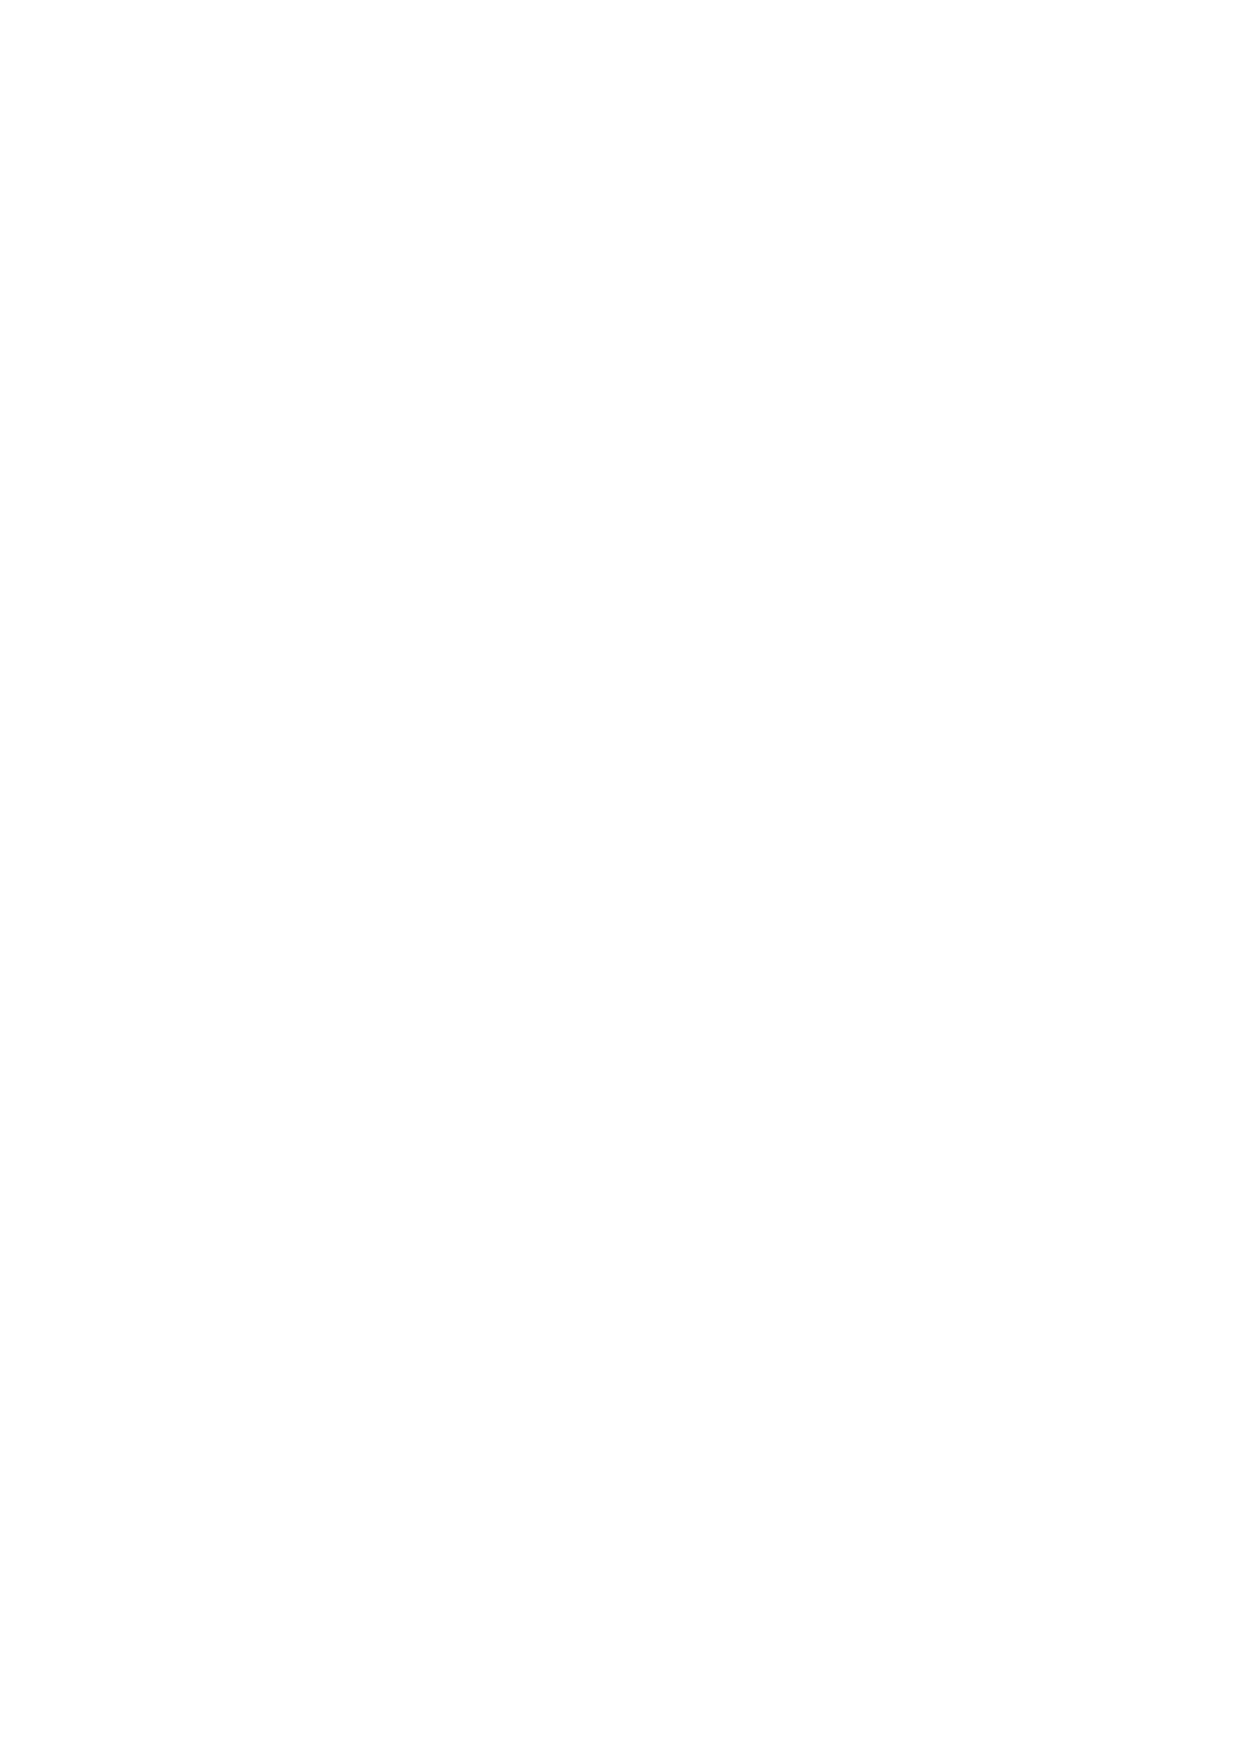
\includegraphics [scale=1.4]{jtr315}
			\caption{Graph of the function $F_{0}$.}
			\label{fig:3.15}
		\end{figure}
		
		Thus, it can be seen that in each of the above three situations, the phase portraits are `qualitatively' the same as for the model family \eqref{3.10}. It would be desirable to construct the family $\left\{ h_{\mu}\right\} $ of local homeomorphisms that implement the topological orbital equivalences of the respective phase portraits. It is quite a tedious task (if you take it very seriously) and we will leave it (even in \cite{Ar2} this is skipped).
	\end{enumerate}
\end{proof}

\begin{remark}
	E. Hopf in his original work proved a more general result than Theorem \ref{theo:3.36}. Namely, he left the assumption that $c_3 \neq 0$ (see \cite{MaMc}). He showed the existence of a $1$-parameter family $\gamma _{\nu }$ of periodic solutions for vector fields $v_{\mu (\nu )}(x)$, where $\left( \mathbb{R}_{+},0\right) \ni \nu \longrightarrow \mu (\nu )$ is a smooth reproduction. This claim is called the \textbf{Hopf Bifurcation Theorem}. For example, for the family
	$$
	\dot{z}=\left( \mu +i\right) z=v_{\mu }(z,\bar{z})
	$$
	we have a family of periodic solutions $\gamma _{\nu }=\left\{
	\left\vert z\right\vert ^{2}=\nu \right\} $ for one field $\dot{z}%
	=iz=v_{0}(z,\bar{z})$, i.e.  $\mu (\nu )\equiv 0$.
	
	Arnold \cite{Ar2} often stressed that in the case of $c_{3}\not=0$, the appropriate bifurcations were examined in parallel by A. Andronov \cite{ALG2}. Therefore, the bifurcation of Theorem \ref{theo:3.36} is called the \textbf{Andronov-Hopf Bifurcation}.
\end{remark}

\begin{example}(Zhukovsky glider model).
	Let a plane fly with speed $v$ (which can change) and is raised at an angle $\theta$ to the horizontal (see Figure \ref{fig:3.16}). The following forces operate on the plane: thrust force $F_c$ directed along the plane, gravity force $mg$ directed downwards and air drag force proportional to $v^2$. We distribute the force of gravity on the component along the plane (causing loss of speed) nd in the perpendicular direction (causing downward rotation). So we have the following pair of equations: $m\dot{v}=F_{c}-mg\sin
	\theta -c_{2}v^{2}$ and $mv\dot{\theta}=-mg\cos \theta +c_{2}v^{2}$. Here the constants $c_1$ and $c_2$ depend on several factors that we will not specify (see \cite{BNF}, Chapter 3, Paragr. 3 and \cite{BaLe}, Chapter 14, Paragr. 3, Chapter 15, Paragr. 3). After the appropriate normalization $y=\textrm{const}\cdot v$, we get the following 2-parameter family of vector fields
	\begin{equation}
	\label{3.14}
	\dot{\theta}=(y^{2}-\cos \theta )/y,\text{ \ \ }\dot{y}=\lambda -\mu
	y^{2}-\sin \theta ,
	\end{equation}
	$-\pi /2\leq \theta \leq \pi /2$, $y\geq 0$, with the pole along $\left\{ y=0\right\}$.
	
		\begin{figure}[!ht]
		\centering
		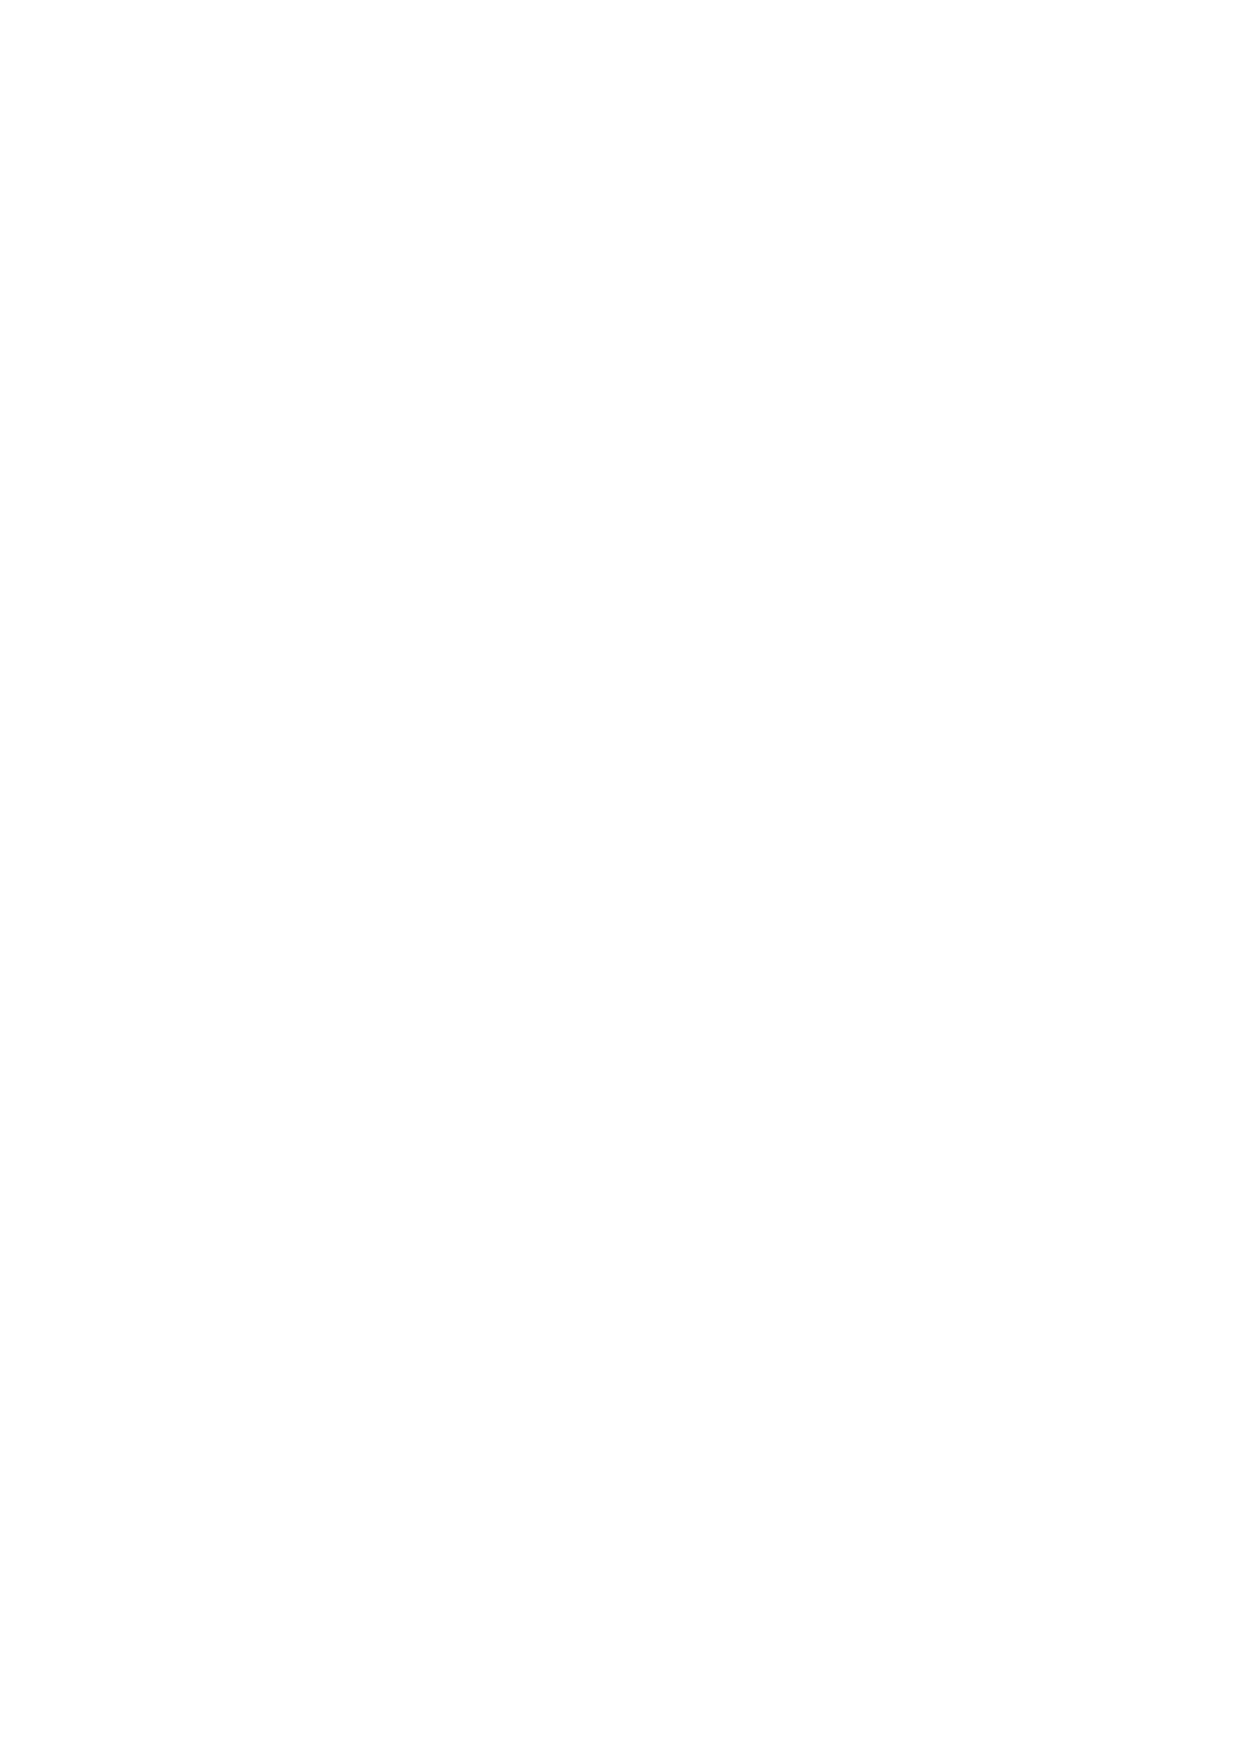
\includegraphics [scale=1.4]{jtr316}
		\caption{Zhukovsky glider.}
		\label{fig:3.16}
	\end{figure}
	
	Let's first consider the case of $\lambda = 0$, which corresponds to the glider model. After multiplying by $y$ (rescaling time) we get a phase portrait of the regular field
	\begin{equation}
	\label{3.15}
	V=(y^{2}-\cos \theta )\partial _{\theta }-y(\sin \theta +\mu y^{2})\partial
	_{y}.
	\end{equation}
	At $\mu =0$ we get the Hamiltonian system with the first integral
	$$
	F=\frac{1}{3}y^{3}-y\cos \theta
	$$
	and the equilibrium points $S_{\pm }=\left( \pm \pi /2,0\right) $ and $C=\left(
	0,1\right) $. With $\mu >0$ we get $\textrm{div}V=-2\mu y<0$, meaning the function $\Phi =y$ is a Dulac function for the field \eqref{3.14}. It is easy to see that for $\mu = 0$, the glider movement is periodic (oscillating around the $C$ center) and for $\mu > 0$ the corresponding critical point $C$ (bifurcating from $(0, 1)$) is a globally stable focus (Task 3.44). This means that the glider's movement is stabilizing.
	
	For the general family \eqref{3.14} with small $\lambda $ and $\mu $, the possible limit cycles can be examined using the abelian integrals method (see Example \eqref{example:4.5} below). The increment $\Delta F$ of the first integral along the trajectory of the system \eqref{3.14} (from cutting to cutting) is approximately
	$$
	\int \dot{F}dt=\int \left( y^{2}-\cos \theta \right) \left( \lambda -\mu
	y^{2}\right) dt\approx \int_{F=c}(\lambda -\mu y^{2})yd\theta =\lambda
	I_{0}(c)-\mu I_{1}(c),
	$$
	where $I_{0}(c)=\int \int dydx$ is the area of the region enclosed by the curve $F(\theta ,y)=c$. In \cite{BaLe} it is shown that the function $c\longmapsto I_{1}(c)/I_{0}(c)$ is monotone, i.e. that the equation $\lambda I_{0}(c)-\mu I_{1}(c)=0$ has at most one solution. This means that the system \eqref{4.14} for small $\lambda $ and $\mu $ can have at most one limit cycle.
	
	Here, at the moment when the field divergence \eqref{3.14} in focus $C$ is zero, the Andronov-Hopf bifurcation takes place. One can check that it is not degenerate (readers are encourage to check this).
\end{example}

\subsection*{Tasks}
\begin{task}
	Show that the coefficients $c_3, c_5,\ldots$ from Point 4 of the assumptions to the Andronov-Hopf Theorem overlap with the Lyapunov-Poincaré focal quantities from Definition \ref{def:2.13}. Find the relationship between the coefficients $c_{2j+1}$ and $d_{2j+1}$ and between $a_{j}$ and
	$b_{j}$.
\end{task}

\begin{task}
	Prove formula \eqref{3.11}.
	
	Tip: Reductions of the finite number of resonant words can be performed simultaneously for a 1-parameter family.
\end{task}

\begin{task}
	Prove formula \eqref{3.12}.
\end{task}

\begin{task}
	Show strictly that the equation $F = 0$ from the proof of Theorem \ref{theo:3.36} has exactly two solutions.
\end{task}

\begin{task}
	Examine the singular points of the field \eqref{3.15}. Sketch phase portraits for $\mu = 0$ and $\mu \neq 0$.
\end{task}

\subsection{Limit cycle bifurcations}
Let $\gamma \subset M$ be a closed phase curve of the vector field $v_{0}(x)$ on the manifold $M$ ($n$-dimensional). In addition, the field $v_{0}(x)$ is immersed in the 1-parameter family $v_{\mu }(x)$, $\mu \in \left( \mathbb{R},0\right)$, of vector fields on $M$. Take the section $S$ transversal  to $\gamma$ in $M$. For $\mu$ close to 0 we get a family of Poincaré return maps $P_{\mu }:S\longmapsto S.$ By identifying $S$ with $\left( \mathbb{R}%
^{n-1},0\right)$, we get a family of local transformations
$$
f_{\mu }:\left( \mathbb{R}^{n-1},0\right) \longmapsto \left( \mathbb{R}%
^{n-1},0\right) ,\text{ \ \ }f_{\mu }(z)=f(z;\mu ),
$$
such that $f_{0}(0)=0.$ So
$$
f_{0}(z)=Az+\ldots
$$
\begin{figure}[!ht]
	\centering
	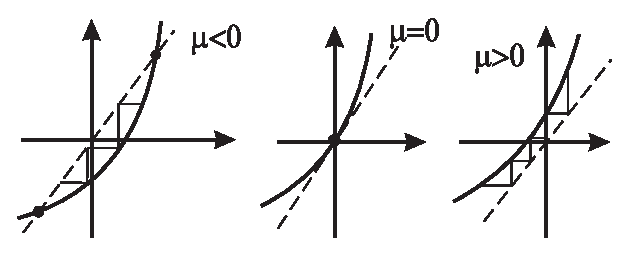
\includegraphics [scale=1.4]{jtr317}
	\caption{Bifurcation of the saddle-node for diffeomorphisms.}
	\label{fig:3.17}
\end{figure}
We also assume that for $\mu =0$ the orbit is non-hyperbolic, i.e. the constant point $z=0$ of the diffeomorphism $f_{0}$ is non-hyperbolic. Depending on the type of hyperbolic we have different types of bifurcations. We will discuss only two here.
\begin{enumerate}
	\item [\textbf{A.}]\textbf{Saddle-node bifurcation for a limit cycle.} Here we have $\lambda _{1}=1$ and $\left\vert \lambda _{j}\right\vert \not=1$ $(j>1)$ for the eigenvalues of the matrix $A$. Bringing situations to the central manifold (i.e. 1-dimensional for diffeomorphism) and applying appropriate conditions of non-degeneration (i.e. $\frac{\partial
	^{2}f}{\partial z^{2}}(0;0)$, $\frac{\partial f}{\partial \mu }(0;0)$ $\not=0)$, we reduce the situation to a 1-dimensional family following the model
	$$
	f(z;\mu) = z+\mu \pm z^2.
	$$
	
	The appropriate bifurcations are shown in Figure \ref{fig:3.17}. We see that for $\mu <0$ we have two limit cycles that merge at $\mu =0$ and then disappear.
	\item [\textbf{B.}]\textbf{Period doubling bifurcation.} Here we have $\lambda _{1}=-1$ and $\left\vert \lambda _{j}\right\vert \not=1$ for $j>1.$ Because the transformation of the return map changes the orientation, the central manifold for the orbit is a Möbius strip (see Figure \ref{fig:3.19}).
	\begin{figure}[!ht]
		\centering
		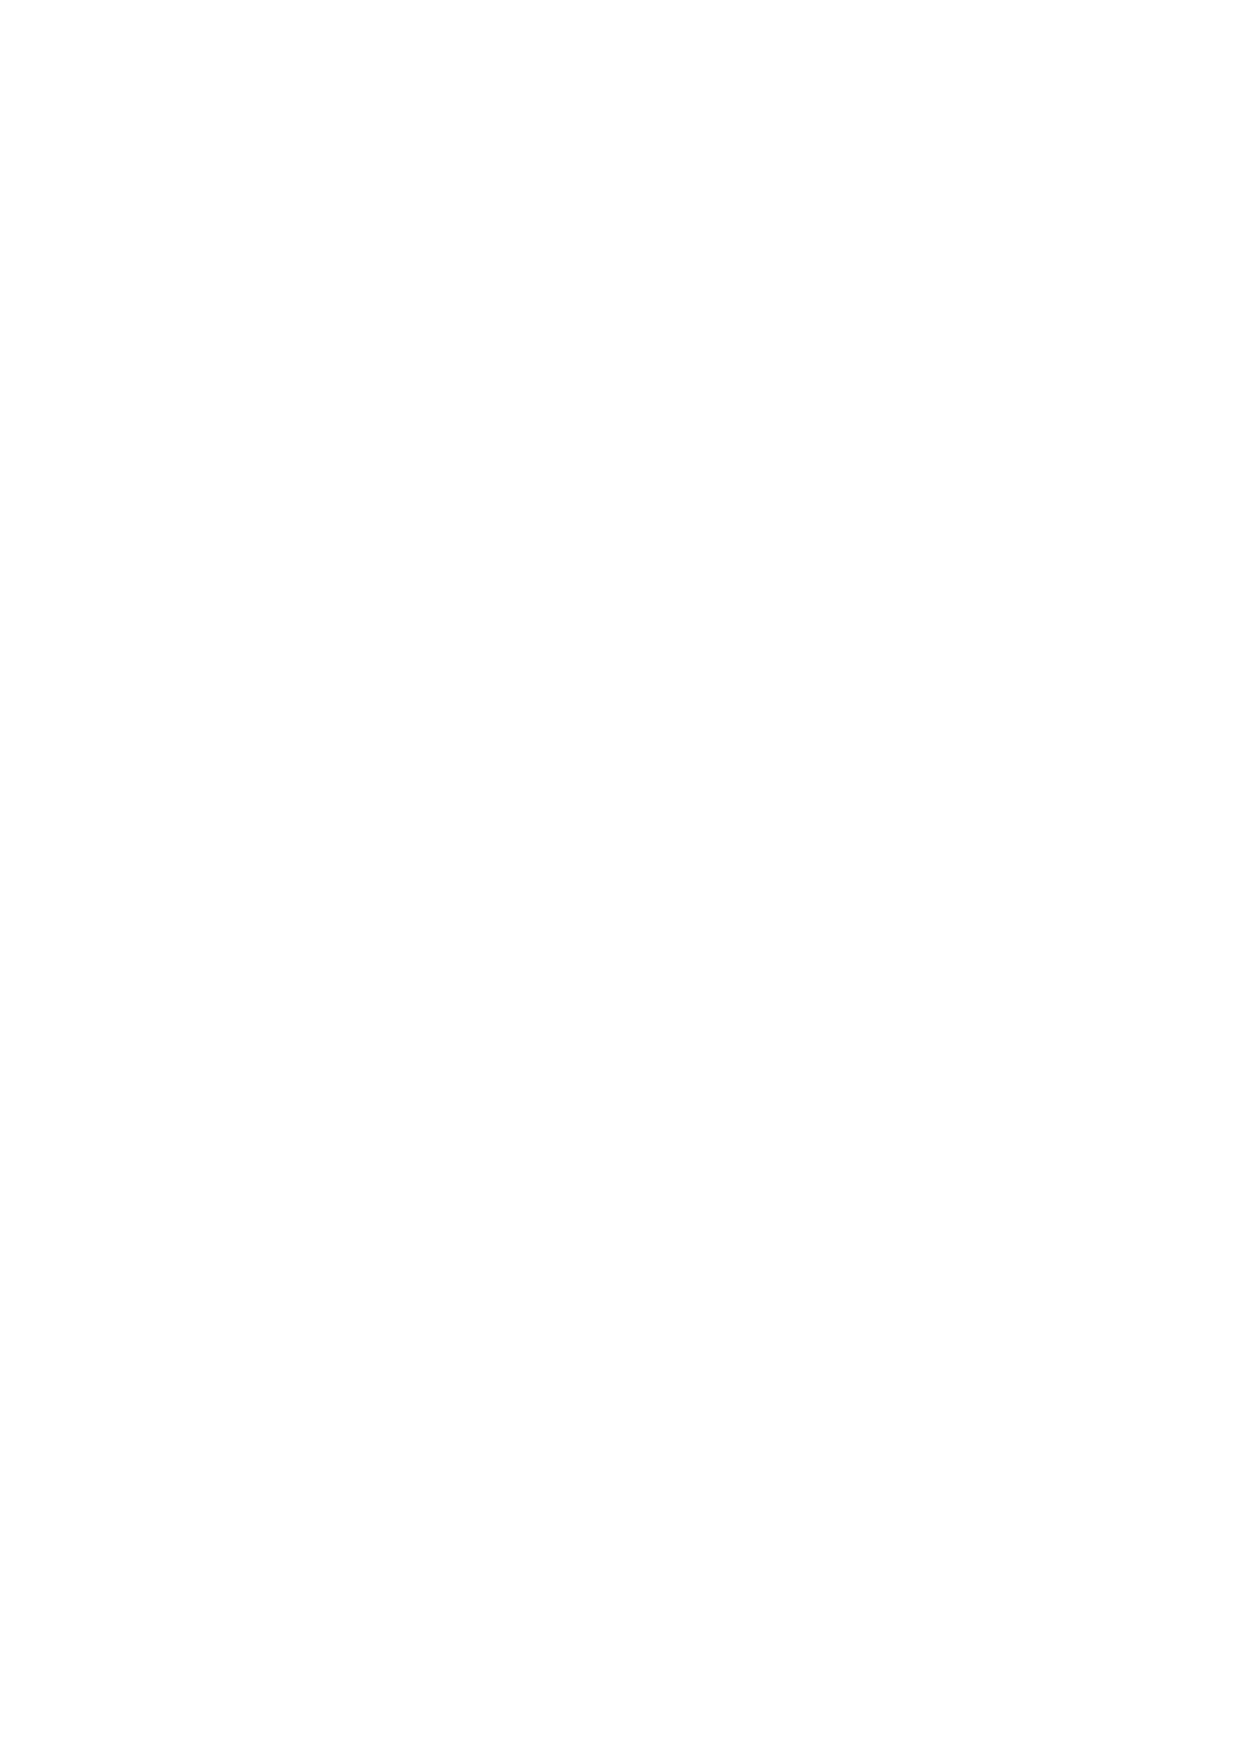
\includegraphics [scale=1.4]{jtr318}
		\caption{Period doubling bifurcation for diffeomorphisms.}
		\label{fig:3.18}
	\end{figure}
	
	The model family transformed in this case is
	$$
	f_{\mu }(z)=f(z,\mu )=\left( -1+\mu \right) z\pm z^{3}.
	$$
	Of course, this transformation has only one fixed point, i.e. $z = 0$. But its second iteration has the form
	$$
	f_{\mu }\circ f_{\mu }(z)=(1-2\mu )z\mp 2z^{3}+\ldots
	$$
	and has two additional fixed points $z_{1,2}\approx \sqrt{\mp \mu }$ for $%
	\mp \mu >0$. These fixed points correspond to the periodic orbit for $f_{\mu}$ with period 2. Thus, the name of bifurcation is taken; sometimes also the name \textit{fork bifurcation} is used (from the shape of the curve of periodic points on the plane$\left( \mu ,z\right)$).
	
	The appropriate bifurcations for $\left\{ f_{\mu }\right\} $ are shown in Figure \ref{fig:3.18}.\footnote{The Period doubling bifurcation lies at the basis of the known Feigenbaum bifurcation for the irreversible transformation of the episode $g:I\longmapsto I$ into itself. First, the fixed point loses stability when passing the eigenvalue by -1. Then there is a periodic period of rotation with period 2 again loses stability and a periodic orbit of period $2^2$ is created, etc. For the parameter's limiting value, we have Feigenbaum bifurcations.}
	
	\begin{figure}[!ht]
		\centering
		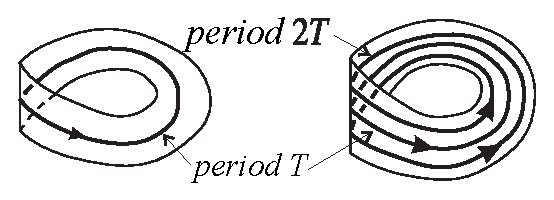
\includegraphics [scale=1.4]{jtr319}
		\caption{Period doubling bifurcation for limit cycles.}
		\label{fig:3.19}
	\end{figure}
\end{enumerate}

On this end we discuss the bifurcation of vector fields. For more details on the bifurcation described above and other bifurcations I refer the readers to literature (\cite{ALG1}, \cite{ALG2}, \cite{Ar2}, \cite{ArPl},
\cite{BaLe}, \cite{BNF}, \cite{GuHo}, \cite{MaMc}).
